% SPDX-License-Identifier: CC-BY-4.0
%
% Copyright (c) 2023 Nelson Vieira
%
% @author Nelson Vieira <2080511@student.uma.pt>
% @contributor Mary Barreto <mary.barreto@staff.uma.pt>
% @license CC-BY-4.0 <https://creativecommons.org/licenses/by/4.0/legalcode.txt>
%
%% Workaround to avoid error:
%%    ! LaTeX Error: Option clash for package xcolor.
%%
%%    The package xcolor has already been loaded with options:
%%    []
%%    There has now been an attempt to load it with options
%%    [divpsnames]
\PassOptionsToPackage{dvipsnames}{xcolor}
\documentclass[runningheads]{llncs}

\RequirePackage{amsmath} % Fixes warning
\RequirePackage{adjustbox}
\RequirePackage{colortbl}
\RequirePackage{tikz}

\setcounter{secnumdepth}{5}
\setcounter{tocdepth}{5}

\usepackage[document]{ragged2e}
\usepackage[nottoc]{tocbibind}
\usepackage[utf8]{inputenc}
\usepackage[T1]{fontenc}
\usepackage[portuguese, english]{babel}
\usepackage[shortlabels]{enumitem}
% \usepackage{a4wide}
\usepackage[hidelinks]{hyperref}
\usepackage{nomencl}
\usepackage{float}
\usepackage{graphicx}
\usepackage{array}
\usepackage{tablefootnote} % table footnotes
\usepackage{url}
% \usepackage[hyphenbreaks]{breakurl} % disabled to fix warning
% \usepackage{lineno}
\usepackage{setspace}
\usepackage[version=4]{mhchem}
\usepackage[flushleft]{threeparttable}
\usepackage{multirow}
\usepackage{import}
\usepackage{eurosym}
\usepackage{parskip}
\usepackage{cite}
\usepackage{pgfgantt}
\usepackage{amsmath,amssymb,amsfonts}
\usepackage{textcomp}
\usepackage{xcolor}
\usepackage{tabularx} % in the preamble
\usepackage{algorithm}
\usepackage{algpseudocode}
\usepackage{datatool}
\usepackage{datetime}
\usepackage{subcaption}

\usepackage[a4paper, total={15cm, 24cm}]{geometry}

\graphicspath{ {figures/} }
\def\UrlBreaks{\do\/\do-}

\onehalfspacing

%% Fix for the sub sub section
\makeatletter
\renewcommand\subsubsection{\@startsection{subsubsection}{3}{\z@}%
    {-18\p@ \@plus -4\p@ \@minus -4\p@}%
    {4\p@ \@plus 2\p@ \@minus 2\p@}%
    {\normalfont\normalsize\bfseries\boldmath
\rightskip=\z@ \@plus 8em\pretolerance=10000 }}
\renewcommand\paragraph{\@startsection{paragraph}{4}{\z@}%
    {-12\p@ \@plus -4\p@ \@minus -4\p@}%
    {2\p@ \@plus 1\p@ \@minus 1\p@}%
    {\normalfont\normalsize\bfseries\boldmath
\rightskip=\z@ \@plus 8em\pretolerance=10000 }}
\makeatother

\makenomenclature



% makeindex thesis.nlo -s nomencl.ist -o thesis.nls
\begin{document}
    \pagenumbering{roman}
    \selectlanguage{english}

    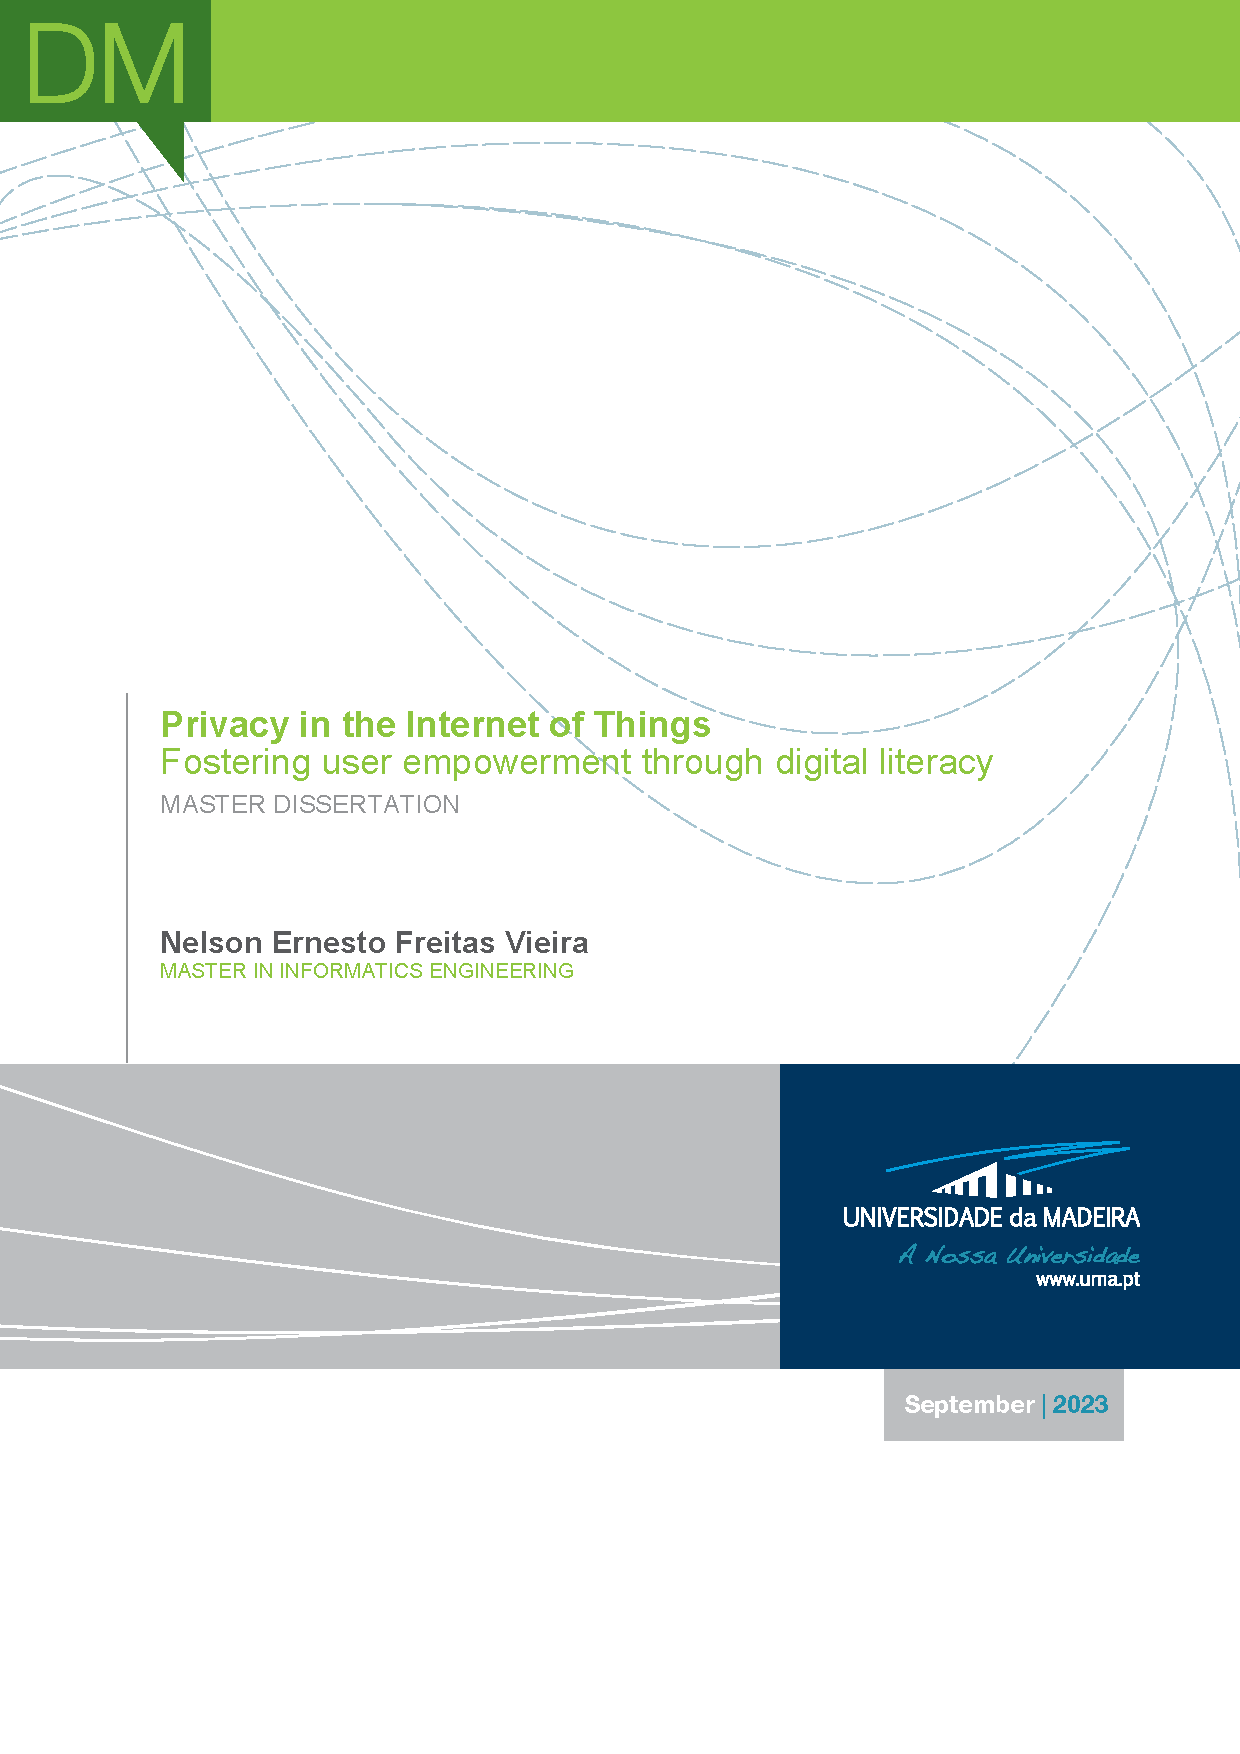
\includepdf[pages=-]{chapters/0_front_cover.pdf}
    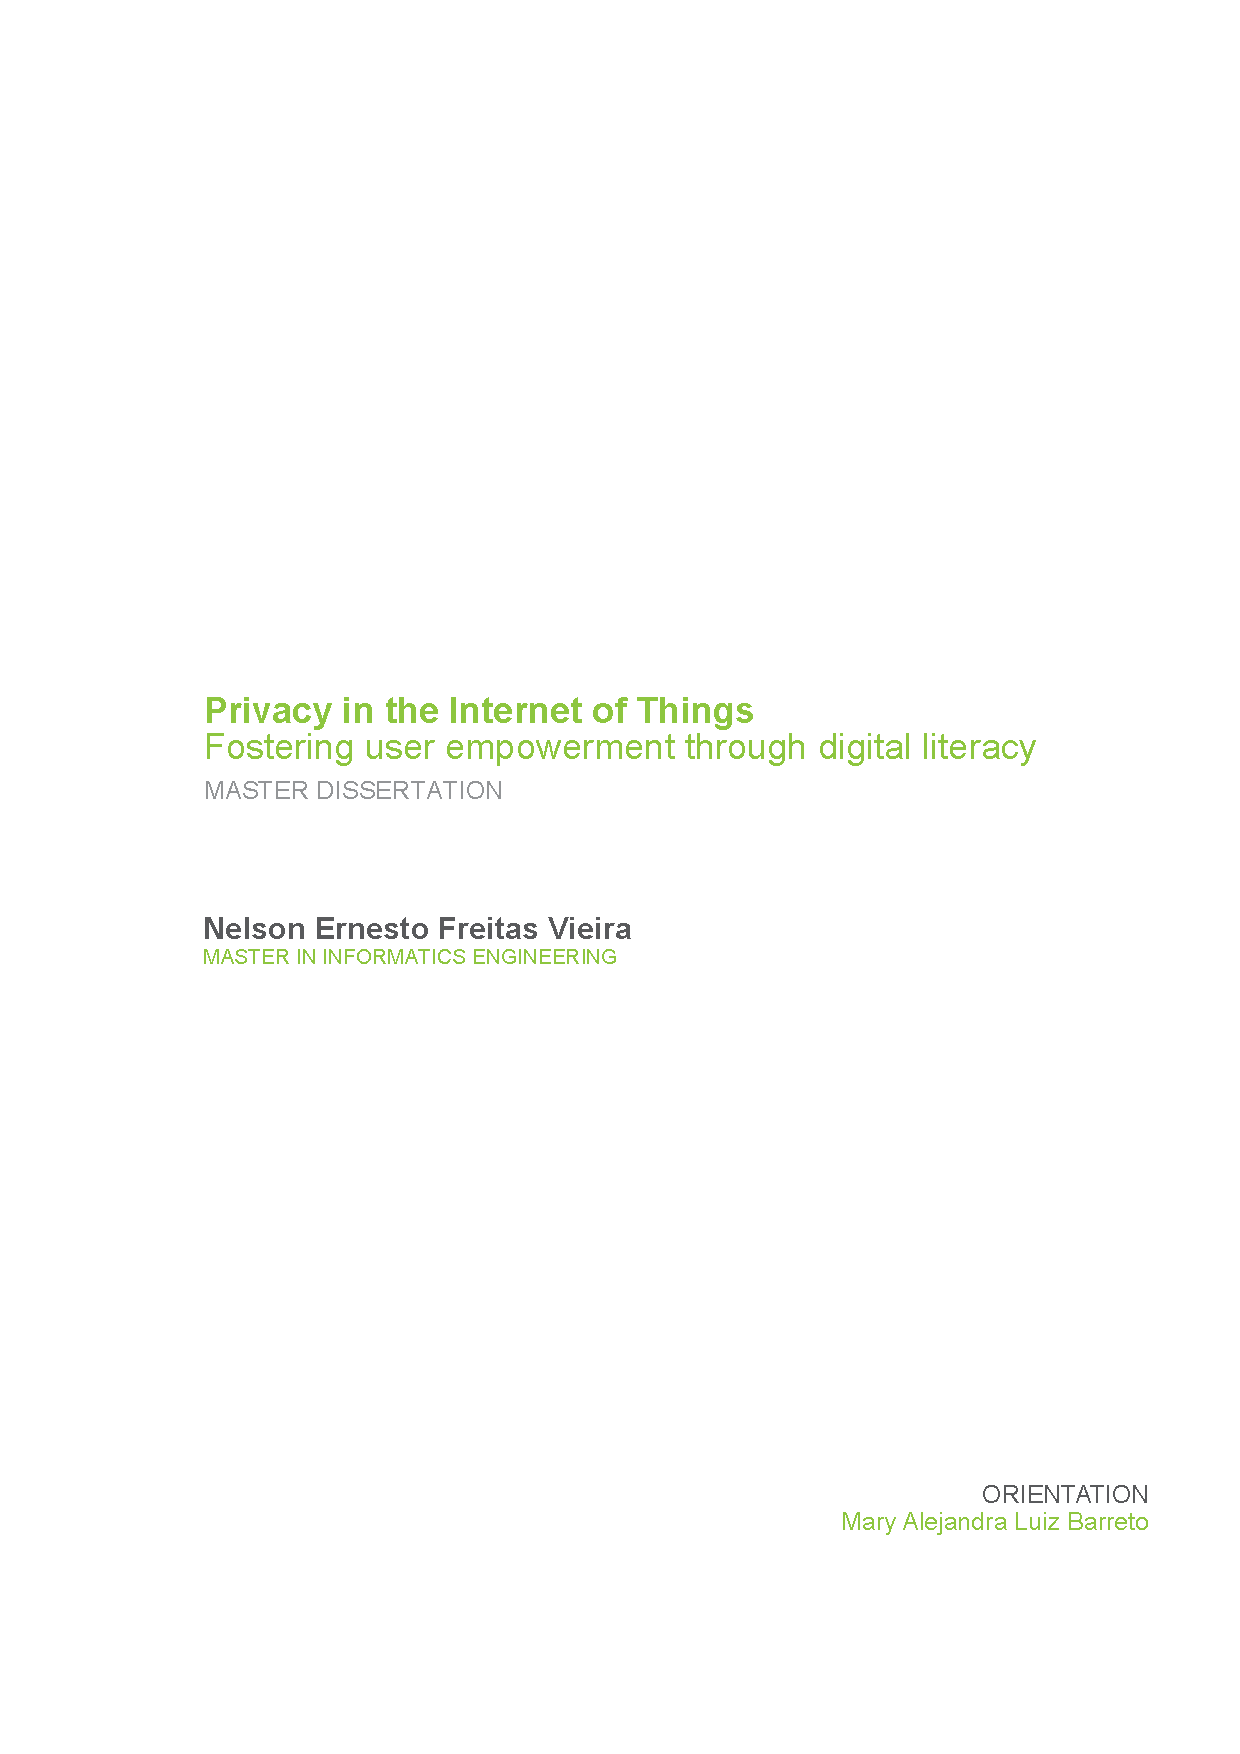
\includepdf[pages=-]{chapters/0_inner_cover.pdf}
    % % SPDX-License-Identifier: CC-BY-4.0
%
% Copyright (c) 2023 Nelson Vieira
%
% @author Nelson Vieira <nelson0.vieira@gmail.com>
% @license CC-BY-4.0 <https://creativecommons.org/licenses/by/4.0/legalcode.txt>
\begin{titlepage}
    \centering
    \addtolength{\hoffset}{0.5cm}
        \centering
        \includegraphics[width=0.50\textwidth]{assets/images/uma_logo.png}\par\vspace{0.5cm}
        {\scshape\LARGE \selectlanguage{portuguese} Faculdade de Ciências Exatas e da Engenharia \par}
        \vspace{1cm}
        {\scshape\Large Mestrado em Engenharia Informática \par}
        \vspace{1.5cm}
        {\huge\bfseries Empowering Users' Privacy Rights in the Internet of Things \par}
        \vspace{2cm}
        {\Large Nelson Ernesto Freitas Vieira\par}
        \vfill
        {\large Orientado por: \par}
            Mary Alejandra Luiz Barreto\par
        \vfill
        {\large Constituição do júri de provas públicas: \par}
            Nome completo (categoria), Presidente \par
            Nome completo (categoria), Vogal \par
            Nome completo (categoria), Vogal \par
        \vfill
    % Bottom of the page
        {\large \bfseries \today \par}
    \end{titlepage}

    % SPDX-License-Identifier: CC-BY-4.0
%
% Copyright (c) 2023 Nelson Vieira
%
% @author Nelson Vieira <2080511@student.uma.pt>
% @license CC-BY-4.0 <https://creativecommons.org/licenses/by/4.0/legalcode.txt>
\chapter*{Resumo}
\justify

Os dispositivos da Internet das Coisas estão por todo o lado, desde
o nascimento da computação ubíqua que se prevê que a vida quotidiana
do ser humano contenha milhões de dispositivos que controlam todos os
aspectos da nossa vida. Hoje em dia, temos veículos inteligentes, casas
inteligentes, cidades inteligentes, dispositivos vestíveis, entre
outros, que utilizam vários tipos de dispositivos e vários tipos de
redes para comunicar. Estes dispositivos criam novas formas de recolha
e tratamento de dados pessoais de utilizadores e não utilizadores.
A maioria dos utilizadores finais nem sequer tem conhecimento ou tem
pouco controlo sobre a informação que está a ser recolhida por
estes sistemas. Este trabalho adopta uma abordagem holística a este
problema, começando por realizar uma revisão da literatura para
compilar as soluções actuais, os desafios e as oportunidades de
investigação futura. Realizando, em seguida, um inquérito para saber mais
sobre o conhecimento geral dos indivíduos acerca da privacidade, da Internet das Coisas e
hábitos \textit{online} e, finalmente, com base na informação recolhida,
é proposta uma aplicação móvel que fornece aos utilizadores informações
sobre os dispositivos que estão próximos e como proteger os dados
que não querem partilhar com estes dispositivos.
Os testes com utilizadores revelaram que os participantes valorizam
ter acesso a mais informações sobre termos relacionados com a privacidade.
Esta aplicação é capaz de detetar que tipo de dispositivos estão próximos,
que tipo de dados são recolhidos por esses dispositivos
e apresentar opções de privacidade ao utilizador, quando possível,
com o objetivo de fornecer aos indivíduos uma ferramenta para tomarem
decisões informadas sobre os seus dados privados.

\keywords{privacidade \and Internet das Coisas \and computação ubíqua \and desafios na IoC \and literacia digital}

    % SPDX-License-Identifier: CC-BY-4.0
%
% Copyright (c) 2023 Nelson Vieira
%
% @author Nelson Vieira <2080511@student.uma.pt>
% @contributor Mary Barreto <mary.barreto@staff.uma.pt>
% @license CC-BY-4.0 <https://creativecommons.org/licenses/by/4.0/legalcode.txt>
\chapter*{Abstract}
\justify

Internet of Things devices are everywhere, since the birth of ubiquitous
computing, human everyday life is expected to contain millions of
devices that control every aspect of our lives. Today we have smart vehicles,
smart houses, smart cities, wearables among other things that use various
types of devices, and various types of networks to communicate. These devices
create new ways of collecting and processing personal data from users, and
non-users. Most end users are not even aware or have little control over
the information that is being collected by these systems. This work takes
a holistic approach to this problem by first conducting a literature review
to compile current solutions, challenges and future research opportunities.
Then conducting a survey to learn more about the general knowledge of
individuals about privacy, IoT and online habits, and finally, based on the
information gathered, a mobile application is proposed that gives users
information about nearby devices, and how
to protect the data that they do not want to share with them.
User testing revealed that participants valued having access to more
information about privacy related terms. This
application is capable of detecting what type of devices are nearby, what kind
of data is collected by these devices, and displaying privacy options to the user,
when it is possible to do so, with the goal of providing individuals a tool to make
informed decisions about their private data.

\keywords{privacy \and Internet of Things \and ubiquitous computing \and challenges in IoT \and digital literacy}

    % SPDX-License-Identifier: CC-BY-4.0
%
% Copyright (c) 2023 Nelson Vieira
%
% @author Nelson Vieira <2080511@student.uma.pt>
% @license CC-BY-4.0 <https://creativecommons.org/licenses/by/4.0/legalcode.txt>
\chapter*{Acknowledgments}

I would like to express my gratitude to my supervisor, Prof. Mary Barreto, for
all the support given, since the initial idea for this dissertation until its conclusion,
the feedback I received was invaluable during the whole process.

I want to thank Prof. Amândio Azevedo for his invaluable insights in the beginning phase of
this work.

I want to give a special thank you to all the people who volunteered to
participate in both the questionnaire and the usability tests, without them this work
would not be possible. Their perspective on privacy and the Internet of Things helped
tremendously during the course of this project, specifically on the development of the application.

Last but not least, I want to thank all the people who supported me during this
process, in particular, my friends that helped to alleviate the difficulties faced and
my family who always supported me. A special thank you goes out to my mother,
who always gave me motivation to continue forward.


    \bfseries
    \tableofcontents
    \normalfont

    \listoffigures

    \listoftables

    % SPDX-License-Identifier: CC-BY-4.0
%
% Copyright (c) 2023 Nelson Vieira
%
% @author Nelson Vieira <nelson0.vieira@gmail.com>
% @license CC-BY-4.0 <https://creativecommons.org/licenses/by/4.0/legalcode.txt>
\chapter*[Acronyms]{List of Acronyms}

% Source: https://latex.org/forum/viewtopic.php?t=16419

% Define a convenient command to add a line
% to the database
\newcommand*{\addacronym}[2]{%
    \DTLnewrow{acronyms}%
    \DTLnewdbentry{acronyms}{Acronym}{#1}%
    \DTLnewdbentry{acronyms}{Description}{#2}%
}

% Create the database
\DTLnewdb{acronyms}
\addacronym{IoT}{Internet of Things}
\addacronym{RFID}{Radio-frequency identification}
\addacronym{MIT}{Massachusetts Institute of Technology}
\addacronym{M2M}{Machine-to-machine}
\addacronym{IP}{Internet Protocol}
\addacronym{GDPR}{General data protection regulation}
\addacronym{CCPA}{California consumer privacy act}
\addacronym{SLR}{Systematic literature review}
\addacronym{PA}{Privacy assistant}
\addacronym{PPA}{Personalized privacy assistant}
\addacronym{SaaS}{Software as a service}
\addacronym{VPN}{Virtual private network}
\addacronym{IT}{Information technology}
\addacronym{VM}{Virtual Machine}
\addacronym{NIST}{National Institute of Standards and Technology}
\addacronym{ISO}{International Organization for Standardization}
\addacronym{RQ}{Research question}
\addacronym{DP}{Differential privacy}
\addacronym{BASE}{Bielefeld Academic Search Engine}
\addacronym{PbD}{Privacy-by-Design}
\addacronym{AI}{Artificial Intelligence}
\addacronym{ICT}{Information and communications technology}
\addacronym{RIA}{Regulatory impact assessment}
\addacronym{EU}{European Union}
\addacronym{DPDCM}{Double-projection deep computation model}
\addacronym{PPDPDCM}{Privacy-preserving double-projection deep computation model}
\addacronym{DCM}{Deep computation model}
\addacronym{LDP}{Local differential privacy}
\addacronym{CCTV}{Closed-circuit television}
\addacronym{USA}{United States of America}
\addacronym{UK}{United Kingdom}
\addacronym{SUS}{System Usability Scale}

% Sort the database
\DTLsort{Acronym}{acronyms}

% Display the contents of the database
\begin{itemize}
\DTLforeach*{acronyms}{\thisAcronym=Acronym,\thisDesc=Description}%
    {\item[] \textbf{\thisAcronym} \thisDesc}%
\end{itemize}


    %% Fix for the nomenclature spacing
    \newlength{\nomitemorigsep}
    \setlength{\nomitemorigsep}{\nomitemsep}
    \setlength{\nomitemsep}{-\parsep}
    \newcommand\bparagraph[1]{\vspace{1.0mm}\noindent\textbf{#1.}}
    \hypertarget{abbr}{\printnomenclature{}}
    \clearpage

    \setcounter{page}{1}
    \pagenumbering{arabic}
    % \linenumbers
    % SPDX-License-Identifier: CC-BY-4.0
%
% Copyright (c) 2023 Nelson Vieira
%
% @author Nelson Vieira <nelson0.vieira@gmail.com>
% @license CC-BY-4.0 <https://creativecommons.org/licenses/by/4.0/legalcode.txt>
\section{Introduction} \label{introduction}

Privacy as we know it is a somewhat recent concept \cite{vincent2016privacy, moore2017privacy},
before the digital age there was barely any notion of privacy for most
people. For many centuries most people used to reside in small communities
where they were continuously involved in one another's lives. Even more
recent is the idea that privacy is a crucial component of personal security,
in contrast to the undeniable necessity of public security, including the
requirement for guarded walls and closed doors. Long seen as a luxury, privacy
is still usually regarded as a good to have rather than an essential
requirement, even though it is acknowledged as a human right, as present
in article 12 of the Universal Declaration of Human Rights \cite{RooseveltUniversal}:
``No one shall be subjected to arbitrary interference with his privacy,
family, home or correspondence, nor to attacks upon his honour and reputation.
Everyone has the right to the protection of the law against such interference
or attacks''. Privacy can be defined \cite{InternationalWhat, SpiekermannEngineering}
as the right to govern how personal information and data is collected, stored,
and used, it frequently involves handling sensitive information with care,
and as such, organizations must be open and honest about the kind of data
they plan to gather, why they need it, and where and with whom they plan
to share it. Users should have the right to control their shared information.

This definition can cause some confusion with the idea of security \cite{HIVDifference}
and although privacy and security are interconnected, security involves
measures taken to safeguard data from risk, threat or danger, it frequently
alludes to safety. It is the practice of keeping users' personal information
and data safe and preventing unauthorized access to it. The primary contrast
between privacy and security is that the former deals with personal information
to individuals and how they want their data used and maintained, whilst
the latter deals with its protection from possible threats. Security can
exist without privacy, but the opposite is not true. For managing sensitive
and personal data, privacy and computer security are equally crucial. Users
should be aware of the internal procedures regarding the collection, processing,
retention, and sharing of personal information.

Concerns about digital privacy have been growing \cite{emami2019exploring, park2022personal, zhang2022peer}
in the last few years, especially after the Anonymous decentralized hacker
group cyber attacks, WikiLeaks and Snowden's leaked top secret documents
from United State's National Security Agency. These concerns can be noted
with the increase of written literature on the subject, when searching for
terms like ``privacy'', ``online privacy'', ``digital privacy'' in Google
Scholar, ACM Digital Library or Science Direct it can be seen that, in the
last 5 years, it returns about 5000000, 650000 and 80000 documents respectively,
including articles, books, conference papers etc.

Most research has focused on the web, while privacy in IoT systems has not
been explored as much. Because IoT devices are becoming more prevalent,
new methods of communicating, gathering, and analyzing data emerge.
Because there is already a substantial quantity of research focusing on
web privacy rather than IoT privacy, it is a lot more fertile ground to
explore the issue of privacy in the context of the IoT.

\textit{Internet of Things} is a term that first appeared in the 1990s,
and it may be linked to Mark Weiser's paper on ubiquitous computing \cite{weiser1991computer}
and the growth of devices of all sizes that communicate with one another
to do various tasks, making Weiser's dream a reality. The first use of the
term \textit{Internet of Things} was in 1999 by British technology pioneer
Kevin Ashton \cite{KevinThat}, executive director of the Auto-ID Center
at Massachusetts Institute of Technology (MIT), to describe a system in
which items may be connected to the internet by sensors. He came up with
the phrase while giving a presentation for Procter \& Gamble to highlight
the value of linking Radio-Frequency Identification (RFID) tags used in
corporate supply chains to the internet in order to count and track goods
without the need for human assistance. These devices are used in various
applications, starting at home \cite{marikyan2019systematic} with thermostats,
fridges, microwaves, etc, moving on to smart cars \cite{arena2020overview},
the educational system \cite{al2020survey}, our clothes and our watches \cite{niknejad2020comprehensive}
and even into outer space \cite{AkyildizInternet}. IoT resources may include
IoT equipment (like smart home assistants and autonomous vehicles), IoT
services (like video analytics services linked to smart cameras and indoor
position tracking systems), or IoT apps (like smart TV remote apps) that
track and use information about us. Internet of Things is now widely used
to describe situations in which a range of objects, gadgets, sensors, and
ordinary items are connected to the internet and have computational capabilities.

The idea of using computers and networks in order to monitor and manage
devices is nothing new, despite the term \textit{Internet of Things} being
relatively recent.
% By the late 1970s, technologies for remotely monitoring electricity
% grid meters through telephone lines were already in use in the corporate
% sector \cite{}.
Wireless technology improvements in the 1990s permitted the widespread
adoption of corporate and industrial machine-to-machine (M2M) solutions
for equipment monitoring and operation. Many early M2M solutions, on the
other hand, relied on proprietary purpose-built networks or industry-specific
standards rather than internet standards. To connect devices other than
computers to the internet is not a new concept. A Coke machine at Carnegie
Mellon University's Computer Science Department \cite{EverhartInteresting}
was the first ubiquitous device to be linked to the internet. The system,
which was created in 1982, remotely observed the out of stock lights on
the pressing buttons of the vending machine and broadcast the state of each
row of the vending machine on the network so that it could be accessed using
the Name/Finger protocol through a terminal. In 1990, a toaster that could
be turned on and off over the internet that was created by John Romkey \cite{RomkeyToast},
was demonstrated at the Interop Internet Networking show.

% \cite{rose2015internet}
% The term "Internet of Things" (IoT) was first used in 1999 by British technology
% pioneer Kevin Ashton to describe a system in which objects in the physical world
% could be connected to the Internet by sensors.12 Ashton coined the term to
% illustrate the power of connecting Radio-Frequency Identification (RFID) tags13
% used in corporate supply chains to the Internet in order to count and track goods
% without the need for human intervention. Today, the Internet of Things has become
% a popular term for describing scenarios in which Internet connectivity and computing
% capability extend to a variety of objects, devices, sensors, and everyday items.

% While the term "Internet of Things" is relatively new, the concept of combining
% computers and networks to monitor and control devices has been around for decades.
% By the late 1970s, for example, systems for remotely monitoring meters on the
% electrical grid via telephone lines were already in commercial use. In the
% 1990s, advances in wireless technology allowed "machine-to-machine" (M2M)
% enterprise and industrial solutions for equipment monitoring and operation to
% become widespread. Many of these early M2M solutions, however, were based on closed
% purpose-built networks and proprietary or industry-specific standards, rather than
% on Internet Protocol (IP)-based networks and Internet standards. Using IP to connect
% devices other than computers to the Internet is not a new idea. The first Internet
% "device"—an IP-enabled toaster that could be turned on and off over the Internet—was
% featured at an Internet conference in 1990. Over the next several years, other
% "things" were IP-enabled, including a soda machine at Carnegie Mellon University in
% the US and a coffee pot in the Trojan Room at the University of Cambridge in the UK
% (which remained Internet-connected until 2001). From these whimsical beginnings, a
% robust field of research and development into "smart object networking" helped
% create the foundation for today's Internet of Things.

The Internet of Things can be defined as: ``An open and comprehensive network
of intelligent objects that have the capacity to auto-organize, share information,
data and resources, reacting and acting in face of situations and changes
in the environment'' \cite{madakam2015internet}.

IoT is one of the fastest growing technologies \cite{MohammadState}, it
is predicted that it will grow into the trillions of devices by 2030 \cite{SarawiInternet},
and with this expansion new security vulnerabilities and data gathering
dangers appear, the lack of security in these devices makes them ideal targets
for privacy violations and inadequate customer disclosure of device capabilities
and data practices aggravates privacy and security issues.

Privacy in IoT systems in not seen as a crucial factor in development \cite{alhirabi2021security}.
Specific standards for privacy options have been imposed by data privacy
regulations including the General Data Protection Regulation (GDPR) and
California Consumer Privacy Act (CCPA), but even these regulations have
been criticized \cite{peloquin2020disruptive, gladis2022weaponizing, gentile2022deficient, green2022flaws, byun2019privacy}.

% TODO: integrate this part in the text

When the first computers were being built, privacy was not even considered
a concern because they were being used for calculations, with the Turing
machine being a seminal influence, only on the following decades when computers
became connected with each other that slowly privacy came to the forefront. In
1973, the US Department of Health, Education, and Welfare published \textit{Records,
Computers and the Rights of Citizens, Report of the Secretary's Advisory
Committee on Automated Personal Data Systems} \cite{hew1973records}, one of the
first documents on digital privacy and an important first step that would
form the basis for modern privacy legislation. In 1977 a revision of privacy
policies would be published by the Privacy Protection Study Commission \cite{united1977personal}.
Meanwhile in the 1980's computers were becoming more ubiquitous in workplaces
and gaining popularity in people's homes but still not much discussion was
happening regarding digital privacy. With the introduction of the World Wide
Web at the start of the following decade, privacy concerns began to increase.

Privacy has become such an important concern in the information (and many
times disinformation) age that we live because most computer/technology/web
organizations heavily rely on the advertising industry which in turn
relies on consumer data. Many organizations after the 2000's provided
their services to the public without an initial cost, because the consumer
does not have to pay to access the service and because the organization
needs income so stay afloat the consumer ends up being used as a commodity
for their data.

    \clearpage
    % SPDX-License-Identifier: CC-BY-4.0
%
% Copyright (c) 2023 Nelson Vieira
%
% @author Nelson Vieira <nelson0.vieira@gmail.com>
% @license CC-BY-4.0 <https://creativecommons.org/licenses/by/4.0/legalcode.txt>
\section{State of the Art}

\par
This section provides an overview of the recent literature with the themes
that were found to be more relevant for this work.

\subsection{Privacy Paradox}

The use of a variety of digital devices have numerous advantages, but they
also bring with them the ubiquity of data capturing equipment, therefore,
it is understandable why the majority of online users have serious concerns
about the privacy of their personal data. However, the opinions expressed
are starkly at odds with the reality, according to Thomson et al. \cite{DarrenState}
report on the state of privacy, that just one in four European users read
the terms and conditions in their entirety prior to making an online purchase
or subscribing to a service, 59\% admitted to only quickly scanning the
terms and conditions before completing a purchase, while 14\% admitted to
never reading them at all, 30\% of the respondents would even swap their
email address to win a reward, or entry into a raffle, while 17\% would do
so to get an app and 30\% would do it for money.

This is what is called a privacy paradox, there have been multiple papers
written on this subject \cite{solove2021myth, WilliamsPrivacy, lee2021investigating, goad2021privacy, gerber2018explaining},
some papers attempt a theoretical explanation while others attempt an empirical
one. There has been very different interpretations or explanations of this
paradox, a few papers \cite{wilson2012unpacking, warshaw2015can, lee2015privacy}
apply the theoretical concept of the \textit{homo economicus} \cite{zak2008moral},
which is the representation of people as beings who constantly act in a
way that is logical and self-interested, not worrying about morality or
ethics, and who do so to the best of their ability, to the context of privacy.
Different cognitive biases and heuristics can influence how consumers make
decisions, according to several studies on consumer choice behavior \cite{acquisti2007can, knijnenburg2013dimensionality, wakefield2013influence, flender2012type}.
According to several articles \cite{dienlin2015privacy, baek2014solving},
this paradox might be explained by the fact that some people have genuinely
experienced online privacy assaults and that most privacy views are therefore
based on heuristics or secondhand accounts. Taddicken's study \cite{taddicken2014privacy}
argues that peer pressure is the reason people have this contradictory behavior,
Norberg et al. \cite{norberg2007privacy} explains this paradox by suggesting
that while perceived risk affects reported attitudes and behavioral intentions,
trust has a direct impact on privacy behavior, while others \cite{flender2012type, kokolakis2017privacy}
rely on quantum theory. Brandimarte et al. \cite{brandimarte2013misplaced}
have explored the idea that when it comes to their data privacy, users have
an \textit{illusion of control}.

This paradox has been proven to be vitiated by a number of empirical studies \cite{dienlin2015privacy, xie2019consumers, SCHWAIG20131, sannon2018privacy},
online privacy practices are founded on separate privacy mindsets and so
they are not inherently paradoxical.

\subsection{Privacy in IoT: Approaches}

There have been a number of systematic literature reviews (SLR) \cite{Gupta2022Privacy, Kuhtreiber2022survey, sicari2015security, LinSurvey}
and systematic mapping reviews \cite{porras2018security, ahmed2019aspects}
done to study privacy and security issues in IoT.

In Gupta and Ghanavati's \cite{Gupta2022Privacy} SLR, the authors review
papers with methodologies and techniques that identify privacy risks or
notify users about these risks. They divide the literature into the following
categories: `Ontological Modeling and Semantic-based Approaches', `Data-Driven
Approaches', `Source Code Analysis-based Approaches', `User Studies and
Survey-based Approaches', `Blockchain-based Approaches' and `Architectural
and Framework-based Approaches'. They then examine current literature on
these three prerequisites. The findings show that: most works concentrate
on single IoT devices when addressing privacy threats; When analyzing privacy
issues, key privacy factors such as data reduction and data aggregation
are overlooked; existing studies ignored the sensitivity of the obtained
information; most useful studies did not include a diverse range of users
when assessing privacy problems; no work has been done to discover compliance
difficulties between an IoT application and different privacy rules; and
current research does not place a premium on providing consumers with real-time
privacy notices. However, this SLR has the following limitations: the authors
only chose articles and not thesis or books and from the selected papers,
only the ones written in english were considered.

% Kühtreiber et al. \cite{Kuhtreiber2022survey} conduct a survey of the frameworks
% and tools created for developers, particularly in the case of IoT, and they conclude
% that present solutions are difficult to use, only effective in specific circumstances,
% and insufficient to address the privacy problems inherent in IoT development. This
% study lacks a comprehensive gap analysis of the chosen literature and it does not
% specify the research questions that define the relevancy of the selected papers.

% Kühtreiber et al. \cite{Kuhtreiber2022survey} evaluate the frameworks and tools
% established for developers, notably in the case of IoT, and find that current
% solutions are difficult to use, only successful in limited contexts, and insufficient
% to handle the privacy issues inherent in IoT development. This study lacks a detailed
% gap analysis of the selected literature, as well as the research questions that
% characterize the relevance of the selected publications.

Kühtreiber et al. \cite{Kuhtreiber2022survey} evaluate the frameworks and
tools established for developers, specifically in the case of IoT, and find
that current solutions are difficult to use, only successful in limited
scenarios, and insufficient to handle the privacy problems inherent in IoT
development. This study lacks a comprehensive gap review of the chosen
literature, along with research questions establishing the significance
of the articles chosen.

% Sicari et al. \cite{sicari2015security} conduct an analysis of recent studies and
% active initiatives that emphasize IoT privacy and security solutions. They begin
% by outlining the needs for IoT privacy and security, including access control,
% confidentiality, and authentication. They then review the literature that already
% exists in relation to these three needs. They concluded that IoT privacy concerns
% are only partially investigated and need further attention. The study, however,
% has its shortcomings, the analysis of prior research focuses primarily on security
% needs and leaves out privacy considerations, they don't perform a thorough gap
% analysis on the publications that were examined, and they don't provide a thorough
% summary of the future research topics in the field of IoT privacy that need more
% attention.

% Sicari et al. \cite{sicari2015security} examine current research and ongoing activities
% that focus on IoT privacy and security solutions. They start by stating the
% requirements for IoT privacy and security, such as access control, confidentiality,
% and authentication. They next go over the existing literature in connection to these
% three needs. They came to the conclusion that IoT privacy risks have only been
% partially examined and require more attention. The study, however, has flaws: the
% analysis of prior research focuses primarily on security needs and ignores privacy
% considerations; they do not perform a thorough gap analysis on the publications
% examined; and they do not provide a comprehensive summary of future research topics
% in the field of IoT privacy that require more attention.

Sicari et al. \cite{sicari2015security} examine current research and ongoing
activities that focus on IoT privacy and security solutions. The authors
start by describing the requirements for IoT privacy and security, such
as access control, confidentiality, and authentication. The authors then
conduct a literature study in connection to these three needs. The authors
came to the conclusion that IoT privacy issues have only been partially
examined and that further attention is required. The study, however, has
flaws: the prior research analysis focuses primarily on security needs while
ignoring privacy considerations; the authors do not conduct a thorough gap
analysis on the publications examined; and they do not provide a comprehensive
summary of future research topics in the field of IoT privacy that require
more attention.

% Lin et al. \cite{LinSurvey} undertake a literature review to find security and
% privacy concerns in the network layer, perception layer, and application layer,
% the three IoT architectural layers. Confidentiality, integrity, availability,
% identity and authentication, privacy, and trust are the first six essential security
% properties that the authors list for these levels. Then, for each of the three
% tiers, they examine a number of security attacks. They conclude by providing a
% brief overview of a number of privacy-preserving data procedures, including data
% gathering, data aggregations, and data analysis stages. They do, however, primarily
% focus on the security elements of the IoT and see privacy as one of the most important
% security characteristics, as was already established. Additionally, a thorough gap
% analysis to determine the shortcomings of the previous works is not done in the
% research.

Lin et al. \cite{LinSurvey} undertake a literature review to identify security
and privacy vulnerabilities in the three IoT architecture layers: network,
perception, and application. The authors describe the first six fundamental
security properties for these tiers as confidentiality, integrity, availability,
identification and authentication, privacy, and trust. Then, the authors
look at a variety of security threats for each of the three stages. The
authors wrap up by giving a succinct summary of many privacy-preserving
data techniques, including the stages of data collection, data aggregation,
and data analysis. The authors do, however, largely focus on the IoT's security
components and, as was already said, consider privacy to be one of the most
crucial security aspects, rather than viewing privacy as a distinct concern.
Furthermore, the research does not conduct a thorough gap analysis to discover
the weaknesses of prior efforts.

% Lin et al. \cite{LinSurvey} conduct a literature research to identify security and
% privacy issues in IoT architecture's three levels: network, perception, and
% application. The authors describe the first six fundamental security features
% for these tiers as confidentiality, integrity, availability, identification and
% authentication, privacy, and trust. They next investigate a variety of security
% concerns for each of the three processes. The authors end by offering a succinct
% review of a number of privacy-preserving data methodologies, including data
% collecting, aggregation, and analysis. They do, however, focus mostly on IoT
% security features, and, as previously said, they see privacy as one of the most
% essential security issues. Furthermore, the study did not undertake a detailed gap
% analysis to identify the shortcomings of previous studies.

Based on Ziegeldorf's \cite{ziegeldorf2014privacy} analysis of the literature,
the following are the most prominent privacy concerns in IoT:

\begin{enumerate}
    \item
    The most prominent concern is \textit{identification}, which binds an
    identifier, such as a name and location, with an individual's identity,
    this also enables and aggravates other threats;
    \item
    \textit{Localization and tracking} is the threat of detecting an individual's
    locations through numerous techniques, such as GPS, internet traffic,
    or smartphone location. This threat requires \textit{identification}
    of some kind;
    \item
    In e-commerce, \textit{profiling} is often used for personalization.
    Organizations collect information about individuals in order to deduce
    their interests via association with other profiles and data sources.
    \item
    \textit{Interaction and presentation} allude to the sharing of private
    information with an unintended audience while doing so through a public
    medium. IoT applications often need extensive user interaction, it is
    expected that users of these systems will obtain information via smart
    devices in their immediate surroundings and that users will interface
    with systems in creative, natural ways. However, many of those modes
    of communication and presentation are already available to the broader
    public, making them apparent to anybody around. When personal information
    is transferred between a system and its user, privacy is breached.
    \item
    \textit{Lifecycle transitions} occur when an IoT device is sold, utilized
    by its owner and eventually disposed of. There may be an expectation
    that the object deletes all information, yet smart devices frequently
    keep massive volumes of data about their own past throughout their entire
    existence. This might contain personal images and videos, which are
    not always erased following ownership transfer.
    \item
    \textit{Inventory attacks} involve unauthorized entry and the acquisition
    of information about the presence and characteristics of personal things.
    Malicious users might use inventory data to profile the property and
    break in.
    \item
    \textit{Linkage} is the process of connecting disparate systems, when
    systems are connecting different data sources, there is a higher danger
    of unauthorized access and data leakage.
\end{enumerate}

Another concept worth analyzing is differential privacy which relates more
closely to the survey that will be conducted but also to the general
collection and analysis of user data by applications and systems.

\subsection{Differential Privacy}

The notion of differential privacy, according to Michael Kearns \cite{kearns2019ethical},
is based on three important principles. The first being that ``differential
privacy requires that adding or removing the data record of a single individual
not change the probability of any outcome by much''. The second principle
being that ``no outside observer can learn very much about any individual
because of that person's specific data''. The third important principle
being that ``for every individual in the dataset, and for any observer no
matter what their initial beliefs about the world were, after observing
the output of a differentially private computation, their posterior belief
about anything is close to what it would have been had they observed the
output of the same computation run without the individual's data''.

Differential privacy has the potential to significantly increase individual
privacy protection, by purposefully adding noise into a dataset, it gives
plausible deniability to any individual who may have had their data exploited
while still being able to calculate statistics with relatively high precision.
Although algorithms that deal with notions of fairness, ethics, and privacy
are hard to implement because of the subjectivity of these concepts, and
differential privacy algorithms are no different, they can still help in
regards to addressing technology's inherent moral quandaries.

% Differential privacy is an important component of machine learning algorithms
% and massive datasets, and it has the potential to significantly increase
% individual privacy protection. By purposefully adding noise into a dataset,
% we may give plausible deniability to any individual who may have had their
% data exploited to damage them while still being able to calculate critical
% statistics with high precision. While differential privacy has obvious drawbacks,
% as do many algorithms used to address societal issues, the use of automation and
% machine learning to address subjective notions of fairness, ethics, and privacy
% is a tremendously groundbreaking discovery in the world of computation, and is
% moving us as a society closer to addressing technology's inherent moral quandaries.
% Differential privacy is a fundamental aspect of machine learning algorithms and huge datasets that may substantially increase individual privacy protection. We can provide plausible deniability to every individual who may have their data used to harm them by purposely injecting noise into a dataset, while yet being able to calculate required statistics with high accuracy. While differential privacy, like many algorithms used to address societal issues, has obvious drawbacks, the use of automation and machine learning to address subjective notions of fairness, ethics, and privacy is an incredibly groundbreaking discovery in the world of computation, and is moving us as a society closer to addressing the inherent moral dilemmas of technology.
% Differential privacy is a crucial component of machine learning algorithms and massive datasets that has the potential to significantly boost individual privacy protection. By purposefully inserting noise into a dataset, we can give plausible deniability to any individual who may have their data exploited to harm them while still being able to calculate needed statistics with high precision. While differential privacy has obvious drawbacks, as do many algorithms used to address societal issues, the use of automation and machine learning to address subjective notions of fairness, ethics, and privacy is an incredibly groundbreaking discovery in the world of computation, and is moving us as a society closer to addressing the inherent moral dilemmas of technology.
% Differential privacy is a critical component of machine learning algorithms and large datasets, with the potential to greatly improve individual privacy protection. We can provide plausible deniability to any individual who may have their data misused to harm them while still being able to calculate essential statistics with high accuracy by purposely injecting noise into a dataset. While differential privacy has obvious drawbacks, as do many algorithms used to address societal issues, the use of automation and machine learning to address subjective notions of fairness, ethics, and privacy is an incredibly groundbreaking discovery in the world of computation, and is moving us as a society closer to addressing technology's inherent moral dilemmas.

There exist other algorithms that aim to preserve privacy in the same way
as differential privacy such as Google's box blurring algorithm \cite{FromeLarge}
that is used in the Google Map's street view, Microsoft's Visor \cite{poddar2020visor}
which is a video-analytics-as-a-service tool and Shokri and Shmatikov's
\cite{ShokriPrivacy} system for collaborative deep learning, however, in
general, these algorithms struggle with high computational cost, internal
attacks, or non-provable privacy.

% Zhao et al. \cite{ZhaoSurvey} conduct a SLR on differential privacy
% for unstructured data. The authors present differential privacy methods
% for sensitive content in image, audio, video and text data, they compare
% the various methods and do an utility analysis for each method showing
% the pros and cons of each, the utility loss is measured between the real
% data and its obfuscated version in the experimental evaluations. They
% conclude that differential privacy and its variants have provided
% rigorous privacy guarantees for unstructured data against adversaries
% with arbitrary background information. They also provide possible future
% research topics that have yet to be explored.

Zhao et al. \cite{ZhaoSurvey} conduct a SLR on differential privacy for
unstructured data. The authors present differential privacy methods for
sensitive content in image, audio, video, and text data. They compare the
various methods and perform utility analyses for each method, highlighting
the benefits and drawbacks of each, the utility loss is measured in experimental
evaluations between the actual data and its obfuscated variant. They come
to the conclusion that differential privacy as well as its variations give
stringent privacy protections for unstructured data against attackers with
unpredictable background knowledge. They also suggest potential future study
subjects that have yet to be investigated.

% Privacy concerns arise with the millions of real-world unstructured data including
% images, audios, videos, and texts. Differential privacy has emerged as a de facto
% standard to protect a wide range of data types.
% This article has presented
% differential privacy methods for sensitive content in these unstructured
% data. We have identified that unstructured data are obfuscated based on
% appropriate vector representations, specific privacy models, and vector
% reconstructions. We have discussed possible challenges faced with these
% privacy methods. We have provided an overview of privacy guarantees and
% utility losses in these methods and possible approaches to improve data utility.

% DP and its variants have provided rigorous privacy guarantees for
% unstructured data against adversaries with arbitrary background information.
% While privacy loss has been quantified with the ε value, the utility
% loss is measured between the real data and its obfuscated version in
% the experimental evaluations. Different utility loss metrics are
% adopted to quantify utility losses in different data types. Besides,
% it has been shown that other privacy-protecting methods for unstructured
% data are commonly vulnerable to machine-learning-model-based attacks.
% It is crucial to identify whether DP methods can do away with these
% AI attacks.

\subsection{Título subsecção}

ABC

\subsection{Título subsecção}

ABC

\subsection{Título subsecção}

ABC

    \clearpage
    % SPDX-License-Identifier: CC-BY-4.0
%
% Copyright (c) 2023 Nelson Vieira
%
% @author Nelson Vieira <nelson0.vieira@gmail.com>
% @license CC-BY-4.0 <https://creativecommons.org/licenses/by/4.0/legalcode.txt>
\section{Methodology} \label{section:methodology}

The overall work is comprised of two phases which will be described
in the following paragraphs. The first phase, which is primarily described
on Chapter \ref{section:state_of_the_art}, focuses on gathering the state
of the art in terms of the most relevant topics, from which the main privacy
concepts were selected to be explored in the first stage of phase two with
the creation of a questionnaire with the aim to collect user perceptions
of privacy. The second stage of phase 2 consisted in developing an
application, partially based on the information generated by the survey,
that can identify what sort of devices are around, what kind of data is
gathered by these devices, present privacy options to the user when available,
and what can be done to prevent undesirable data from being collected.
\par
The first phase involved conducting a systematic literature review to gather
the most relevant papers discussing methodologies and techniques for the
protection of user privacy data with a focus on IoT systems. This SLR focused
on papers from the last 13 years, from 2010 until 2023, since papers
published prior to 2010 become out of date with the evolution of technology.
Although certain aspects of privacy have remained constant throughout the years,
this historical perspective on privacy is primarily discussed in the
introduction to this work.

The SLR followed Keshav's three-pass approach \cite{KeshavHow} and
PRISMA 2020 \cite{pagen2021prisma} guidelines when selecting the papers
for review, the principles suggested by Kitchenham and Charters \cite{kitchenham2007guidelines}
were also taken into account in order to ensure the transparency and
reliability of the review. On Keshav's approach, first the title would
be read, then the abstract, the introduction and conclusion and briefly
skim the rest of the paper and then decide if it was worth reading any
further. If the document passed the inclusion criteria, which will be
discussed further ahead, then the document would be read in its entirety
while ignoring any tables, figures, images or graphs. If the paper failed
to present any interesting idea, approach, or technique it would be discarded,
but if not, it would be read carefully from the beginning again in order
to fully understand what it presents.
% Figure \ref{} represents this process.

It is challenging to curate the literature and
gain an in-depth understanding of its different aspects due to the vast
array of approaches that address the topic IoT privacy. As a result, specific
databases were used because of the sheer quantity of papers contained within
them makes research easier. The following were the primary databases of the SLR:

\begin{itemize}
    \item[$\bullet$]
    Google Scholar;
    \item[$\bullet$]
    ScienceDirect;
    \item[$\bullet$]
    IEEE Explore Digital Library;
    \item[$\bullet$]
    ResearchGate;
    \item[$\bullet$]
    Elicit;
    \item[$\bullet$]
    BASE.
\end{itemize}

Other supplementary databases used, during the course of the research, include:
CORE, AIS, ACM Digital Library, Semantic Scholar, Baidu Scholar, RefSeek and
Science.gov. These databases were used in to search certain works that
would have not been found otherwise.

The papers were collected by searching the databases with keywords, a broad
spectrum of results were obtained using generic terms like. The primary search
terms were used between quotation marks, e.g. ``Internet of Things'', so that
results include all words in sequence, operators AND and OR were also used
as was a minus sign before a keyword to remove said keyword from the search
results. Many search terms were utilized, however the most often
used ones, based on their frequency, include: ``Digital literacy'',
``Differential privacy'', ``Privacy paradox'', ``Machine learning'',
``Blockchain'', ``User awareness'', ``User knowledge'', ``Blockchain'',
``Privacy concerns'', ``Privacy perceptions'', ``Regulation'',
``Framework'', ``Security'', ``Deep learning'', ``Approach''.
Most of these search terms also included the terms ``Privacy'' and/or
``Internet of Things'' or any variants like ``IoT'' or ``IoT privacy''.

The SLR attempts to summarize and evaluate IoT privacy concerns, as well
as ideas, techniques, or methodologies to overcome those challenges.
The focal point in this phase was answering the following question: Does
the paper present a new methodology or interesting angle to tackle users'
privacy concerns?
% A better restatement of inclusion criteria is formulated
% in the following research questions:\\

% \vspace{5mm}
% \textbf{Phase 1 (Literature review):} \\

% \textbf{RQ1:} What approaches are currently being considered to address privacy
% issues in IoT?

% \textbf{RQ2:} What issues are prevalent in IoT that make it challenging to
% protect individuals privacy? \\

As referenced before, only papers published from 2010 until 2023 are considered,
these works must also be published in journals, conference proceedings, dissertations,
thesis or technical reports. Exclusion criteria include: presentations, editorials,
abstracts or commentaries. Works can cover any area as long as they deal with
privacy in the Internet of Things, if the paper does not cover IoT then at least
it must cover privacy aspects that can be applied to IoT, as is the case of the
privacy paradox.

From database searches, a total of 229 papers were found. Applying the inclusion
and exclusion criteria to these papers bring the total number of papers down to
95, excluding 134 papers. After reading the full texts of the remaining 95 papers,
47 were excluded, making the number of total papers in the SRL be 48.

Having collected the major findings of the SLR, this work then aimed to conduct a
throughout study split into two stages, which will compose phase 2 of this work.
% The following research questions will be made for this phase:\\

% \vspace{5mm}
% \textbf{Phase 2 (Survey and application):} \\

% \textbf{RQ3:} What are the perceptions of individuals on online privacy?

% \textbf{RQ4:} How can users be empowered to protect their privacy in IoT systems?\\
% \vspace{5mm}

The second phase was evaluated on two stages, the first one consisted
on doing a questionnaire on people's general privacy concerns, while using and interacting
with IoT devices. The SLR helped on the creation of the questionnaire to
assess general user's knowledge on privacy concepts, their habits and concerns,
their understanding of privacy rights, and what they do to safeguard those
rights. The goal of this study was to both understand the privacy paradox
and collect insights on how to address privacy issues in IoT devices.

% Having collected the major findings, this work then aims to conduct a throughout
% study split in several stages and around the following research questions:

% \textbf{RQ1:} What approaches are being considered for privacy issues in
% IoT in the currently available literature?

% \textbf{RQ2:} What IoT-related tools are available that empower users to
% protect their privacy rights? OR How to empower users to protect their privacy
% rights?

% \textbf{RQ3:} What issues are prevalent in IoT that make it difficult to
% address privacy and security problems?

% The proposed methodology is composed of two phases, the first phase consists
% on doing a study on people's general privacy concerns while using and interacting
% with IoT devices. This study will consist on preparing a questionnaire to
% assess general user's knowledge on privacy concepts, their habits and concerns,
% their understanding of privacy rights, and what they do to safeguard those
% rights. The goal of this study is to both understand the privacy paradox
% and collect data on their proposal to address privacy issues with regard
% to IoT devices. The second phase consists in developing an application, partially
% based on the information generated by the survey, that can identify what sort
% of devices are around, what kind of data is gathered by these devices, present
% privacy options to the user where available, and what can be done to prevent
% undesirable data from being collected.

% The second phase consists
% in doing an application that can detect IoT devices nearby the user with.
% The application should do the following when
% detecting a device:
% 1. it should show some information about the device;
% 2. it should categorize the device;
% 3. it should provide the user with privacy options, if the device allows the
% user to decline data harvesting.
% This application at first sight might appear to be a mere privacy assistant
% but it's not, because IoT assistants merely choose what privacy options the
% user first sets and maintains it for every other application that the user
% might use. The proposed app doesn't have the objective to conform to the user's
% preferred privacy choices, it merely informs the user about nearby IoT devices
% and can provide the user with privacy options. But the main objective is creating
% awareness in individuals about the various devices that are around and make
% the user questions their choices.

\subsection{Stage 1: User perceptions}

This questionnaire aims to understand people's perception of IoT and their privacy
practices online. It also serves to better understand and demystify the privacy
paradox and to help provide a solution to the privacy issue in IoT, which will be
discussed on Section \ref{subsection:stage2}.

The questionnaire consisted of 86 questions divided into 7 sections to
gauge users' digital literacy, the first section being about general privacy
questions, then about the predisposition to data sharing, to concerns with
privacy then about daily digital routines, then about profile identification,
subsequently about IoT general knowledge before a final part about
non-identifiable demographic data. The questionnaire's structure is shown
in more detail in Table \ref{table:questionnaire}, the full questionnaire
is presented on Appendix \ref{appendix:survey}.

\begin{table}[H]
    \begin{center}
        \begin{tabular}{r *{3}{ p{6cm} }}
            \hline
            $\#$\hspace{0.5cm} & Section & Details \\
            \hline
            1\hspace{0.5cm} & General knowledge and attitudes towards privacy & This
            section's goal is to ask generic questions regarding the participants awareness
            of information privacy. \\
            \hline
            2\hspace{0.5cm} & Disposition for sharing personal information & This
            section is designed to elicit generic inquiries about the participants
            willingness to provide personal information. \\
            \hline
            3\hspace{0.5cm} & Privacy concerns & This section strives to
            elicit questions about potential concerns about disclosing
            personal information. \\
            \hline
            4\hspace{0.5cm} & Current online habits and practices & This
            section includes general questions with regard to working with
            the internet in everyday activities. \\
            \hline
            5\hspace{0.5cm} & Profile identification & This section gathers
            more particular questions concerning employing profiles to make
            it more straightforward to generate tailor-made interactions. \\
            \hline
            6\hspace{0.5cm} & Knowledge and habits regarding the Internet
            of Things & This section contains questions about participants'
            usage patterns for IoT devices as well as questions that aim to
            understand their level of literacy. \\
            \hline
            7\hspace{0.5cm} & Demographic data & This section is for
            gathering broad demographic information that allows
            to characterize the participants in statistical terms. \\
            \hline
        \end{tabular}
    \end{center}
    \vspace{1em}
    \caption{Structure of questionnaire}
    \label{table:questionnaire}
\end{table}

Great care was taken when it comes to this questionnaire's data collection, in
order to not identify any individual or group of individuals, for
instance, when it comes to differential privacy, any data that might
identify someone will not be disclosed, even though the data might suffer
from some inaccuracy because of this.

The scale that was used in the questionnaire, which is from one to seven,
is based on the work of Philip K. Masur \cite{masur2018situational}, it
was chosen because it provides a more nuanced understanding
of the knowledge of participants. This scale was developed as an
online privacy concerns scale so it fits perfectly on this questionnaire,
another scale, also developed by Masur with Teutsch and Trepte,
that could be used but was ultimately not chosen is the Online Privacy
Literacy Scale \cite{masur2017entwicklung}, although the questionnaire does
contain some of the main aspects of this scale like knowledge of data collection and
analysis practices by institutions and online service providers
knowledge of data protection law, knowledge of technical aspects of data
protection and knowledge of data protection strategies.
This survey was partially based in a study done in the Philippines by the
government in the context of their privacy act of 2012 \cite{Philippine2022Conduct},
this was the second survey done on the country's population. It was also
inspired by Alves's master's thesis \cite{alves2021}, which was about citizen's
perception about privacy in the wake of GDPR.

This survey was constructed in Google Forms and distributed through the internet,
the intent would be that this would reach as many individuals as possible,
besides Google Forms itself, it was used other online venues for distribution
like social media, forum websites, through in person discussions and
some participants responded when also doing the application usability tests.

The questionnaire was available for completion until August 30, 2023,
and during the time that it was open 46 participants responded.
Several online survey dissemination services were used to acquire participants,
all the services used were based on the goodwill of the participants, there
was no financial incentive for completing the survey. Most of the services
used were software as a service (SaaS), these platforms are based
on credits for filling in other questionnaires available, this makes the process
of acquiring participants very tedious as many questionnaires need to be
filled in to get a reasonable number of participants (at least 150 to
200 participants). Disseminating the questionnaire in this way does not
entail any additional cost, but it may mean that the results obtained
in this way may not be as honest as possible, as some participants may
be filling in this questionnaire quickly just to get the number of participants
for their own questionnaires, but there is also no way to guarantee that
if this questionnaire was carried out with some financial incentive that
participants would fill it in as honestly as possible. In addition to
dissemination by the various services, social networks were also as well
as it was personally disseminated to family and friends. One possible
method of dissemination would be in person, house to house,
but this would be a very slow way to get responses, not to mention that
people might feel obligated to respond, which could be considered to be
unethical, and the answers might have been answered in a less than
honest manner.

From the respondents, 47\% are male and 51\% are female, while 2\% don't identify
as neither, see Figure \ref{fig:genre}. 40\% of the participants are younger
than 25 years old, 31.11\% are aged between 26 and 35, 9\% are between
36 and 45 years old, 18\% are older than 46 but younger than 65 and 2\% are
have more than 65 years, as shown on Figure \ref{fig:age}.

\begin{figure}[H]
    \begin{center}
        \begin{tikzpicture}
            \begin{axis}[
                ybar,
                bar width=20pt,
                ymin=0,
                ymax=60,
                symbolic x coords={Male,Female,Other},
                xtick=data,
                axis x line=bottom,
                axis y line=left,
                enlarge x limits=0.2,
                nodes near coords={\pgfmathprintnumber\pgfplotspointmeta\%}
            ]
                \addplot coordinates {(Male,47) (Female,51) (Other,2)};
            \end{axis}
        \end{tikzpicture}
        \caption{Genre distribution of participants.}
        \label{fig:genre}
    \end{center}
\end{figure}

\begin{figure}[H]
    \begin{center}
        \begin{tikzpicture}
            \begin{axis}[
                ybar,
                bar width=20pt,
                ymin=0,
                ymax=50,
                symbolic x coords={18-25,26-35,36-45,46-65,65+},
                xtick=data,
                axis x line=bottom,
                axis y line=left,
                enlarge x limits=0.2,
                nodes near coords={\pgfmathprintnumber\pgfplotspointmeta\%}
            ]
                \addplot coordinates {(18-25,40) (26-35,31.11) (36-45,8.89) (46-65,17.78) (65+,2.22)};
            \end{axis}
        \end{tikzpicture}
        \caption{Age ranges of participants.}
        \label{fig:age}
    \end{center}
\end{figure}

Most of the respondents have a bachelor's degree, 66.67\% to be exact, 17.78\% have
only finished high school, 2.22\% only have a basic education, 11.11\%
have a master's degree and 2.22\% have a doctorate, as pictured on Figure \ref{fig:education}.

\begin{figure}[H]
    \begin{center}
        \begin{tikzpicture}
            \begin{axis}[
                height=7.5cm,
                width=15cm,
                ybar,
                bar width=20pt,
                ymin=0,
                ymax=70,
                symbolic x coords={Basic education,High school,Bachelor's degree,Master's degree,Doctorate},
                xtick=data,
                axis x line=bottom,
                axis y line=left,
                enlarge x limits=0.1,
                nodes near coords={\pgfmathprintnumber\pgfplotspointmeta\%}
            ]
                \addplot coordinates {(Basic education,2.22) (High school,17.78) (Bachelor's degree,66.67) (Master's degree,11.11) (Doctorate,2.22)};
            \end{axis}
        \end{tikzpicture}
        \caption{Education qualifications distribution of participants.}
        \label{fig:education}
    \end{center}
\end{figure}

\subsection{Stage 2: An application of theory into practice}
\label{subsection:stage2}

This work proposes an application that gives users information about IoT
devices that inhabit their surroundings, like the type of information these devices
collect and what privacy options are available. This application is developed
for mobile phones due to the fact that these are the most used devices
and people take them everywhere they go, this is important because the application
uses georeferencing to show the location of the IoT devices. This application
has two main objectives, the first is to inform and educate users in order improve
their digital literacy on this particular field (privacy on IoT systems, and
IoT in general) and the other being to give users a way to make informed decisions
to protect their private data, in a concise and convenient place. Generally
the application will show the geolocation of the IoT devices, what type of
device it is, what type of data is being collect by the device. The application
will not detect the devices by itself, this will be done by the users themselves,
in the first iterations of the application it was discussed that the application
itself would automatically detect the devices by using some kind of sniffer
and would categorize what type of device it was and what type of data it
was collecting but it was discovered that this approach was too complex and
so it was not feasible to do with the constraints of this thesis. The application
is developed with Flutter, other options considered were React Native or a
progressive web application, but Flutter uses ahead of time and just in time
compilation, with Dart as it is programming language, while React Native uses
the Javascript programming language that was never created for mobile programming,
so it uses a bridge to convert Javascript to native components for Android
or iOS. Flutter has better performance and as such it was the chosen framework
for this application.

The first step before creating any prototypes or starting the development was
creating a software requirements specification, as can be read on Appendix \ref{appendix:software_requirements},
delineating the scope and vision for the application; the involved stakeholders;
containing contextual, data-flow and swimlane diagrams; software requirements, including
business, technology, functional and non-functional requirements; use cases
and requirements prioritisation.

Users can, when they start the application for the first time, freely use it to see
which devices are in their vicinity,
information about the devices, information about the application itself, and
information about privacy in general and more specifically privacy in IoT systems
which they can use to improve their digital literacy. What they cannot do is
add a new device to the application or edit a device's information. The user has
to create an account first to do these operations. The decision to add an
account creation before the user can add or edit a device is to prevent
bad actors to add bogus data to the application making unusable for the majority
of people, this solution doesn't completely solve this issue (because bad actors
can still create an account and add bogus data anyway) but it helps to slow
down the insertion of bad data.

Upon account creation the only data entry that can be considered sensitive that
the user has to input is an email address.
After the user has created an account and logs in, the user can add devices to the application with the following information:

\begin{itemize}
    \item[$\bullet$]
    The \textbf{name of the device}: This serves to differentiate between the various devices on the application and as such should be unique to each device, it is used on various routes and is one of the first fields that users see about a device. A single device does not have an \textit{official} name, what is more probable is that the device has a model name or is part of a system with it's own name. The user creates the name, this could be abused by bad actors but it is extremely discouraged. It is used for aesthetic reasons.
    \item[$\bullet$]
    The \textbf{category of the device}: This is used to categorize each devices main type of information that the device is collecting. These can be of the following:
    \begin{itemize}
        \item[$\circ$] \textbf{Visual}: The device mainly collects visual information with maybe a video camera.
        \item[$\circ$] \textbf{Audio}: The device mainly collects audio information with a sound recorder.
        \item[$\circ$] \textbf{Presence}: The device can detect the presence of nearby objects or persons. This is not the same as the location category because the device does not know the location of an individual, it merely knows that the individual is nearby. These type of devices can be used, for example, to collect information about how many people frequent a specific store.
        \item[$\circ$] \textbf{Location}: The device can detect the exact or approximate location of an individual, it can use GPS to get this kind of information.
        \item[$\circ$] \textbf{Biometrics}: The devices collects biometric data, this can be the number of steps an individual (or animal) takes, or health related data like the heart beat.
        \item[$\circ$] \textbf{Environment}: These type of devices collect environmental data, they can be used for agriculture or weather forecasting by collecting, for example, temperature, humidity or wind speed/direction data.
        \item[$\circ$] \textbf{Unique identification}: This category is for a device that can uniquely identify an individual, the device itself most likely is not capable of doing it but with other information that the device has access to, it can be used to cross reference of information and as such uniquely identify a person. An example of this would be a device a device that can collect visual data and with facial recognition used against other data in a database it can uniquely identify an individual.
    \end{itemize}
    \item[$\bullet$]
    The \textbf{purpose for the data collection}: Defines what is the purpose for the collection of the data, if a device collects temperature and humidity data and is used by a weather based company or government agency then the purpose for the data collection is for weather forecasting.
    \item[$\bullet$]
    \textbf{Who has access to the collected data}: Disclose an individual or group of individuals that have access to the data of the device, if the device is part of a closed system it can be that only an individual as access to the data but most likely various groups of people have access to the data, some with more data than others depending on the permissions they have. If the device publicizes its data then everyone has access to it.
    \item[$\bullet$]
    \textbf{For how long is the data stored}: Pinpoint the duration of the stored data in the device or system, due to legislation passed in various countries this duration has a limit, in some cases the data cannot be stored for more than one year.
    \item[$\bullet$]
    \textbf{Can the data identify anyone}: Used to quickly identify if a particular device can identify an individual or not. If the device belongs to the "Unique identification" category then this should be active.
    \item[$\bullet$]
    \textbf{What is being done with the data}: This could be assumed to be similar to the \textbf{purpose} field mentioned above but it should be used to diagnose what is being done now with the data collected, in certain situations it might coincide with the purpose for the data collection.
    \item[$\bullet$]
    \textbf{Privacy options}: The user can insert an url for the device's privacy options, in some cases the device, or company, has a website with information on privacy options, or privacy policy. If the device uses a mobile application then a link to the this application can be inserted here.
    \item[$\bullet$]
    \textbf{Coordinates of the device}: Used to express the latitude and longitude of the device so that it can be shown on the map, on the homepage of the application.
    \item[$\bullet$]
    \textbf{Who owns the device}: Who is the device owner, if it belongs to an organization then the name of the organization should appear here otherwise if the device belongs to a person then the person's name should \textbf{not} appear, it should say private or something similar.
\end{itemize}

The user is not required to provide information to satisfy all items on this list, the
only information that is required in order to add a device to the application is
the name, category and coordinates of the device, all other
information is optional but should be provided for the sake of guaranteeing a good
experience to other users of the application. The information provided
should be verified by the user beforehand so that bogus data does not clutter
the application, in this case there are no absolute ways of guaranteeing this
but the maintainer of the application edit wrong information or in some
cases remove it, other users can also edit any device data. This is an
open platform so it is expected that users act in good faith.

% Types of data:
% Health
% Visual
% Audio
% Presence (if user is nearby)
% Location (precise location of user)
% Biometrics
% Environment
% Unique identification (with the help of other means)

% Information to be added to the app:
% What is the purpose of the data collection
% Who can access the data
% For how long is it stored
% Can the data identify anyone
% What is done with this data

% \section{Current Stage of the Work}

% The preliminary results of the study, based on 10 responses, show that everyone
% agrees that privacy is important to them and some people know that they
% should not share their personal information with anyone they do not trust
% (like clicking on random urls or using unprotected websites/software), but
% most of them think that privacy and security are the same concept, most
% respondents also do not read privacy notices but accept them to access the
% information they want to get to, most respondents use their devices mostly
% to access social networks and for work, when it comes to IoT, there is a
% dissonance between knowing the term and using devices like smart watches
% or RFID enabled devices, from the respondents that answered yes to using
% IoT devices most use because of work. It is also noted that most respondent
% have a background in engineering, so the responses are skewed. As a result,
% the survey will remain open to gather a larger number of responses and participants
% for more significant results and generalizations.

% \begin{table}[ht]
% \centering
% \begin{adjustbox}{width=0.5\textwidth}
% \small
% \noindent\begin{tabular}{p{0.17\textwidth}*{20}{|p{0.01\textwidth}}|}
% \hline
% \multicolumn{0}{|c|}{Work plan}
%     & \multicolumn{4}{c|}{January}
%     & \multicolumn{4}{c|}{February}
%     & \multicolumn{4}{c|}{March}
%     & \multicolumn{4}{c|}{April}
%     & \multicolumn{4}{c|}{May}
%     \\
% \hline
% \hline
% \multicolumn{0}{|l|}{Week}
%     & 1 & 2 & 3 & 4 & 1 & 2 & 3 & 4& 1 & 2 & 3 & 4& 1 & 2 & 3 & 4& 1 & 2 & 3 & 4 \\
% \hline
% % using the on macro to fill in twenty cells as `on'
% \multicolumn{0}{|l|}{Discovery and planning}
%     & \cellcolor[cmyk]{1,1,0,0}&&&& &&&& &&&& &&&&&&& \\
% \hline
% \multicolumn{0}{|l|}{Research enquiry}
%     & \cellcolor[cmyk]{1,1,0,0} & \cellcolor[cmyk]{1,1,0,0} & \cellcolor[cmyk]{1,1,0,0} & \cellcolor[cmyk]{1,1,0,0} & \cellcolor[cmyk]{1,1,0,0} & \cellcolor[cmyk]{1,1,0,0} & \cellcolor[cmyk]{1,1,0,0} & \cellcolor[cmyk]{1,1,0,0} & \cellcolor[cmyk]{1,1,0,0} & \cellcolor[cmyk]{1,1,0,0} & \cellcolor[cmyk]{1,1,0,0} & \cellcolor[cmyk]{1,1,0,0} &&&& &&&& \\
% \hline
% \multicolumn{0}{|l|}{State of the art}
%     & \cellcolor[cmyk]{1,1,0,0} & \cellcolor[cmyk]{1,1,0,0} & \cellcolor[cmyk]{1,1,0,0} & \cellcolor[cmyk]{1,1,0,0} & \cellcolor[cmyk]{1,1,0,0} & \cellcolor[cmyk]{1,1,0,0} & \cellcolor[cmyk]{1,1,0,0} & \cellcolor[cmyk]{1,1,0,0} &&&& &&&& &&&& \\
% \hline
% \multicolumn{0}{|l|}{Project requirements}
%     & \cellcolor[cmyk]{1,1,0,0} & \cellcolor[cmyk]{1,1,0,0} & \cellcolor[cmyk]{1,1,0,0} & \cellcolor[cmyk]{1,1,0,0} &&&& &&&& &&&& &&&& \\
% \hline
% \multicolumn{0}{|l|}{Wireframes and user stories}
%     &&&& & \cellcolor[cmyk]{1,1,0,0} & \cellcolor[cmyk]{1,1,0,0} & \cellcolor[cmyk]{1,1,0,0} & \cellcolor[cmyk]{1,1,0,0} &&&& &&&& &&&& \\
% \hline
% \multicolumn{0}{|l|}{Prototyping and refinement}
%     &&&&&& && \cellcolor[cmyk]{1,1,0,0} & \cellcolor[cmyk]{1,1,0,0} & \cellcolor[cmyk]{1,1,0,0} & \cellcolor[cmyk]{1,1,0,0} &&&& &&&& &  \\
% \hline
% \multicolumn{0}{|l|}{Development}
%     &&&& &&&& & \cellcolor[cmyk]{1,1,0,0} & \cellcolor[cmyk]{1,1,0,0} & \cellcolor[cmyk]{1,1,0,0} & \cellcolor[cmyk]{1,1,0,0} & \cellcolor[cmyk]{1,1,0,0} & \cellcolor[cmyk]{1,1,0,0} & \cellcolor[cmyk]{1,1,0,0} & \cellcolor[cmyk]{1,1,0,0} & \cellcolor[cmyk]{1,1,0,0} & \cellcolor[cmyk]{1,1,0,0} & \cellcolor[cmyk]{1,1,0,0} & \cellcolor[cmyk]{1,1,0,0} \\
% \hline
% \multicolumn{0}{|l|}{Tests and iterations}
%     &&&& &&&& &&& & \cellcolor[cmyk]{1,1,0,0} & \cellcolor[cmyk]{1,1,0,0} & \cellcolor[cmyk]{1,1,0,0} & \cellcolor[cmyk]{1,1,0,0} & \cellcolor[cmyk]{1,1,0,0} &&&&  \\
% \hline
% \multicolumn{0}{|l|}{Release and documentation}
%     &&&& &&&& &&&& &&&& & \cellcolor[cmyk]{1,1,0,0} & \cellcolor[cmyk]{1,1,0,0} & \cellcolor[cmyk]{1,1,0,0} & \cellcolor[cmyk]{1,1,0,0} \\
% \hline
% \end{tabular}
% \end{adjustbox}
% \vspace{1em}
% \caption{Work plan timeline}
% \label{workchart}
% \end{table}

% As can be seen in Table \ref{workchart}, the first months will involve the
% design of the application and the enquiry of the study followed by the development
% of the application and the synthesis of the study, and finally testing and
% refinement of the application. Because of the exploratory nature of this
% work the application might suffer alterations to the design, specially in
% the testing stage, and also depending on the results of the study.

\begin{figure}
    \centering
    \begin{subfigure}{0.33\textwidth}
        \centering
        \includegraphics[width=130pt]{../assets/images/low_homepage.png}
        \caption{}
        \label{fig:lowhome}
    \end{subfigure}%
    \begin{subfigure}{0.33\textwidth}
        \centering
        \includegraphics[width=130pt]{../assets/images/low_about.png}
        \caption{}
        \label{fig:lowabout}
    \end{subfigure}%
    \begin{subfigure}{0.33\textwidth}
        \centering
        \includegraphics[width=130pt]{../assets/images/low_more_info.png}
        \caption{}
        \label{fig:lowfaq}
    \end{subfigure}%
    \caption{Low level prototype of (a) homepage, (b) about and (c) FAQ pages.}
    \label{fig:lowlevelprototype}
\end{figure}

After creating the software requirements specification, the prototypes were
created. For the creation of the prototypes the following tools were used: Figma
and GIMP.

At first a low level prototype was made in order to understand the
general design and user interaction of the application. Figure \ref{fig:lowlevelprototype}
shows tree pages of the low level prototype, these are the homepage, about
and faq pages, this prototype has a navigation menu on the bottom where the
other pages of the application can be selected along with some information
above the page icons, this information is supposed to be the categories of
the devices, the logic would be that the user could tap one of these categories
and only devices of that category should be displayed on the map. It can
be seen that between the three pages the map stays in the background and
the various pages work like an overlay on the homepage, this would be
changed in subsequent prototype versions.

\begin{figure}
    \centering
    \begin{subfigure}{0.33\textwidth}
        \centering
        \includegraphics[width=130pt]{../assets/images/low_homepage.png}
        \caption{}
        \label{fig:mediumhome}
    \end{subfigure}%
    \begin{subfigure}{0.33\textwidth}
        \centering
        \includegraphics[width=130pt]{../assets/images/low_about.png}
        \caption{}
        \label{fig:mediumabout}
    \end{subfigure}%
    \begin{subfigure}{0.33\textwidth}
        \centering
        \includegraphics[width=130pt]{../assets/images/low_more_info.png}
        \caption{}
        \label{fig:mediumfaq}
    \end{subfigure}%
    \caption{Medium level prototype of (a) homepage, (b) about and (c) FAQ pages.}
    \label{fig:mediumlevelprototype}
\end{figure}

\begin{figure}[H]
    \centering
    \begin{subfigure}{0.33\textwidth}
        \centering
        \includegraphics[width=130pt]{../assets/images/low_homepage.png}
        \caption{}
        \label{fig:highhome}
    \end{subfigure}%
    \begin{subfigure}{0.33\textwidth}
        \centering
        \includegraphics[width=130pt]{../assets/images/low_about.png}
        \caption{}
        \label{fig:highabout}
    \end{subfigure}%
    \begin{subfigure}{0.33\textwidth}
        \centering
        \includegraphics[width=130pt]{../assets/images/low_more_info.png}
        \caption{}
        \label{fig:highfaq}
    \end{subfigure}%
    \caption{High level prototype of (a) homepage, (b) about and (c) FAQ pages.}
    \label{fig:highlevelprototype}
\end{figure}

\begin{figure}[H]
    \centering
    \begin{subfigure}{0.30\textwidth}
        \centering
        \includegraphics[width=120pt]{../assets/images/live_homepage.jpg}
        \caption{}
        \label{fig:highhome}
    \end{subfigure}%
    \begin{subfigure}{0.30\textwidth}
        \centering
        \includegraphics[width=120pt]{../assets/images/live_about.jpg}
        \caption{}
        \label{fig:highabout}
    \end{subfigure}%
    \begin{subfigure}{0.30\textwidth}
        \centering
        \includegraphics[width=120pt]{../assets/images/live_more_info.jpg}
        \caption{}
        \label{fig:highfaq}
    \end{subfigure}%
    \caption{Live version of the application with pages: (a) homepage, (b) about and (c) FAQ pages.}
    \label{fig:live_app}
\end{figure}

Usability tests were conducted in person with 7 participants of different
ages, professional fields and qualifications. Before doing the tests,
some questions were made to gather the general level of digital literacy
related to IoT and privacy, then the participants were asked to fill in the
survey, if they had not done it yet, as this gives some insight into what the
application is about. The usability tests consists of single ease questions
and system usability scale, as can be seen on appendix \ref{appendix:usability_tests}.
The single ease question was used after the participant performed each task, the
participant would answer how difficult they though the task was in a
scale of 1 to 7. The system usability scale was used after the participants
performed all tasks.

    \clearpage
    % SPDX-License-Identifier: CC-BY-4.0
%
% Copyright (c) 2023 Nelson Vieira
%
% @author Nelson Vieira <nelson0.vieira@gmail.com>
% @license CC-BY-4.0 <https://creativecommons.org/licenses/by/4.0/legalcode.txt>
\section{Privacy Challenges}

IoT is a composed of a complex web of architectures, applications and technologies.
In terms of architectures, it can be decomposed in three layers: the perception
layer, the network layer and the application layer.

The perception layer, also known as the sensor layer, interacts with physical
objects and components via smart devices (RFID, sensors, actuators, and
so on). Its key objectives are to connect objects to the IoT network and
to monitor, collect, and analyze status information about these things using
deployed smart devices. This layer can often be unreliable, for instance
with autonomous vehicles where they find it hard to read road signs or to
predict if certain objects are inanimate or not, but this unreliability
also brings privacy even though some of the data might be unusable. Noise
can also be added in this layer to provide extra privacy.

In the network layer there are many competing networks like ZigBee, Z-Wave,
Bluetooth Low Energy, LoRa, Wi-fi, etc., this layer is fragmented specially
in regards to wireless networks and that makes it very difficult to create
an IoT architecture that can use various networks and have the various
devices communicate with each other, even though interoperability is seen
as a very important factor in IoT. Some of these networks are open standard
protocols while others are proprietary and use different protocols of communication,
use different frequencies, different ranges and different data rates. When
creating an IoT architecture the designers often think of how to solve
specific problems and use what is best for the current needs, and the way
that IoT is fragmented doesn't help in providing progress.

The application layer receives data from the network layer and uses it to
execute essential services or operations. This layer, for example, can provide
the storage service to backup incoming data into a database or the analysis
service to analyze received data in order to predict the future state of
physical devices. This layer encompasses a wide range of applications, each
with its own set of requirements. A few examples are smart grids, smart
transportation, and smart cities.

% In the network layer there are many competing networks like ZigBee, Z-wave
% Bluetooth Low Energy, LoRa, Wi-fi, etc., this layer is fragmented specially
% in regards to wireless networks, and that makes it very difficult to create
% an IoT architecture that can use various networks and have the various
% devices communicate with each other, even though interoperability is seen
% as a very important factor in IoT. Some of these networks are free to use
% while others are proprietary and use different protocols of communication,
% use different frequencies, different ranges and different data rates. When
% creating an IoT architecture the designers often think of how to solve
% specific problems and use what is best for the current needs, and the way
% that IoT is fragmented doesn't help in providing progress.
% In the network layer there are many competing networks like ZigBee, Z-wave
% Bluetooth Low Energy, LoRa, Wi-fi, etc., this layer is fragmented specially
% in regards to wireless networks, and that makes it very difficult to create
% an IoT architecture that can use various networks and have the various
% devices communicate with each other, even though interoperability is seen
% as a very important factor in IoT. Some of these networks are free to use
% while others are proprietary and use different protocols of communication,
% use different frequencies, different ranges and different data rates. When
% creating an IoT architecture the designers often think of how to solve
% specific problems and use what is best for the current needs, and the way
% that IoT is fragmented doesn't help in providing progress.

According to Qu et al. \cite{Qu2018Privacy}, several significant barriers
remain, including the lack of a theoretical foundation, the trade-off optimization
between privacy and data value, and system isomerism over-complexity. Because
there are no mathematical foundations for IoT structure design, IoT system
designs are planned and executed using empirical approaches, which have
limitations in IoT development. Scientific theory and quantitative analysis
must enable trade-off optimization, yet, there are multiple parties with
diverse characteristics and requirements, making this optimization highly
challenging. A plethora of standards and protocols add to the unneeded complexity
of system isomerism. Ensuring effective IoT applications with as few resources
as possible implies fewer resources available for privacy protection; however,
lightweight privacy protection cannot meet all of the criteria, and attackers
can exploit structural information to launch multiple concurrent attacks.

% According to Qu et al. \cite{Qu2018Privacy}, several substantial barriers
% remain, including the lack of a theoretical framework, the trade-off optimization
% between privacy and data utility, and system isomerism over-complexity.
% There are no mathematical foundations for IoT structure design, IoT system
% designs are planned and performed using empirical ways, the shortcomings of
% empirical methods limit IoT progress. To begin with, improving IoT performance
% entirely on human experience is tough. Second, developing privacy protection
% systems is difficult without theoretical guidance. Third, opponents may
% utilize this function to increase the success rate of their attacks. Trade-off
% optimization must be supported by scientific theory and quantitative analysis.
% Qu et al. highlight several key challenges that still need to be overcome
% namely the lack of a theoretical foundation, the trade-off optimization between
% privacy and data utility and system isomerism over-complexity. There are no
% mathematical foundations for IoT structure design, IoT system architectures
% are designed and implemented using empirical methods, the disadvantages of
% empirical methods limit the development of IoT. First, it is not easy to
% optimize IoT performance simply based on human experience. Second, it is
% difficult to implement privacy protection mechanisms without theoretical
% guidance. Third, adversaries can utilize this fact and increase the success
% rates of attacks. Trade-off optimization has to be built on scientific theory
% and quantitative analysis. However, there are multiple parties with dynamic
% characteristics and diversified requirements, which greatly complicates this
% optimization. Moreover, a lack of theoretical foundation causes non-uniform
% quantitative measurements and thereby introduces uncertainty into trade-off
% optimization. A massive number of standards and protocols facilitate the over-complication
% of the isomerism of systems. An over-complicated isomerism causes inconveniences
% to communication and system integration. Ensuring effective IoT applications
% without wasting too many resources leaves fewer resources for privacy protection.
% Nevertheless, lightweight privacy protection cannot satisfy all the requirements.
% In addition, adversaries can utilize the structural information to launch various
% and continuous attacks.

    \clearpage
    % SPDX-License-Identifier: CC-BY-4.0
%
% Copyright (c) 2023 Nelson Vieira
%
% @author Nelson Vieira <nelson0.vieira@gmail.com>
% @license CC-BY-4.0 <https://creativecommons.org/licenses/by/4.0/legalcode.txt>

\section{Methodology}

The overall work will be comprised of two phases which will be described
in the following paragraphs. Phase one mainly described throughout this
paper, focuses on collecting the state of the art in terms of the most relevant
topics, from which main privacy concepts were selected to be explored in
the stage 1 of Phase 2 with the preparation of a questionnaire to collect
user perceptions regarding privacy and topics collected in the systematic
literature review. The second stage of Phase 2 consists in developing an
application, partially based on the information generated by the survey,
that can identify what sort of devices are around, what kind of data is
gathered by these devices, present privacy options to the user when available,
and what can be done to prevent undesirable data from being collected.
\par
The Phase 1 Systematic Literature Review gathered the most relevant papers
discussing methodologies and techniques for the protection of users' privacy
data with special focus on IoT systems. For this SLR, this paper considered
focusing only on papers from the last 12 years, from 2010 until 2022, since
papers before then become out of date with the evolution of technology.
In this SLR, it was reviewed 54 papers published in top computer science,
security, privacy and software engineering outlets.

This paper followed Keshav's three-pass approach \cite{KeshavHow} when choosing
which papers to read fully and which ones to ignore, first the title would
be read, then the abstract, the introduction and conclusion and briefly
skim the rest of the paper and then decide if it was worth reading any further,
the focal point in this phase was answering the following question: does
the paper present a new methodology or interesting angle to tackle users'
privacy concerns? Only then the document would be read in its entirety while
ignoring any tables, figures, images or graphs. If the paper failed to present
any interesting idea, approach, or technique it would be discarded, but
if not, it would be read carefully from the beginning again in order to
fully understand what it presents. Having collected the major findings,
this work then aims to conduct a throughout study split in several stages
and around the specific research questions which will be explored in each
phase. For that matter, the research questions listed are:

\vspace{5mm}
\textbf{Phase 1:} \\
% \vfill

\textbf{RQ1:} What approaches are being considered for privacy issues in
IoT in the currently available literature?

\textbf{RQ2:} What are user perceptions on online privacy? \\

% \vspace{5mm}
\textbf{Phase 2:} \\
% \vfill

\textbf{RQ3:}
% What IoT-related tools are available that empower users to
% protect their privacy rights? OR
How to empower users to protect their privacy rights?

\textbf{RQ4:} What issues are prevalent in IoT that make it difficult to
address privacy and security problems?
\vspace{5mm}

The second phase will be evaluated on two stages, the first one consists
on doing a study on people's general privacy concerns, while using and interacting
with IoT devices. This study will abide on preparing a questionnaire to
assess general user's knowledge on privacy concepts, their habits and concerns,
their understanding of privacy rights, and what they do to safeguard those
rights. The goal of this study is to both understand the privacy paradox
and collect data on their proposal to address privacy issues with regard
to IoT devices.

% Having collected the major findings, this work then aims to conduct a throughout
% study split in several stages and around the following research questions:

% \textbf{RQ1:} What approaches are being considered for privacy issues in
% IoT in the currently available literature?

% \textbf{RQ2:} What IoT-related tools are available that empower users to
% protect their privacy rights? OR How to empower users to protect their privacy
% rights?

% \textbf{RQ3:} What issues are prevalent in IoT that make it difficult to
% address privacy and security problems?

% The proposed methodology is composed of two phases, the first phase consists
% on doing a study on people's general privacy concerns while using and interacting
% with IoT devices. This study will consist on preparing a questionnaire to
% assess general user's knowledge on privacy concepts, their habits and concerns,
% their understanding of privacy rights, and what they do to safeguard those
% rights. The goal of this study is to both understand the privacy paradox
% and collect data on their proposal to address privacy issues with regard
% to IoT devices. The second phase consists in developing an application, partially
% based on the information generated by the survey, that can identify what sort
% of devices are around, what kind of data is gathered by these devices, present
% privacy options to the user where available, and what can be done to prevent
% undesirable data from being collected.

% The second phase consists
% in doing an application that can detect IoT devices nearby the user with
% at least a 10 meters radius. The application should do the following when
% detecting a device:
% 1. it should show some information about the device;
% 2. it should categorize the device;
% 3. it should provide the user with privacy options, if the device allows the
% user to decline data harvesting.
% This application at first sight might appear to be a mere privacy assistant
% but it's not, because IoT assistants merely choose what privacy options the
% user first sets and maintains it for every other application that the user
% might use. The proposed app doesn't have the objective to conform to the user's
% preferred privacy choices, it merely informs the user about nearby IoT devices
% and can provide the user with privacy options. But the main objective is creating
% awareness in individuals about the various devices that are around and make
% the user questions their choices.

\subsection{Stage 1: User perceptions}

This study aims to understand people's perception of IoT and their privacy
practices online. It also serves to demystify the privacy paradox and also
to help provide a solution to the privacy issue in IoT. The questionnaire
consists of 92 questions divided into 7 sections to access users' knowledge,
it follows a kind of narrative, the first section being general privacy
questions then about the predisposition to data sharing, to concerns with
privacy then about daily digital routines, then about profile identification,
and then about IoT general knowledge before a section about non-identifiable
demographic data. The scale that is used in the questionnaire is based on
the work of Philip K. Masur \cite{masur2018situational}. Great care is taken
when it comes to this survey's data collection, in order to not identify
any individual or group of individuals, for instance, when it comes to differential
privacy, any data that might identify someone will not be disclosed, even
though the data might suffer from some inaccuracy because of this.

This survey was partially based in a study done in the Philippines by the
government in the context of their privacy act of 2012 \cite{Philippine2022Conduct},
this was the second survey done on the country's population. It was also
inspired by Alves's master's thesis \cite{alves2021}, which was about citizen's
perception about privacy in the wake of GDPR.

This survey was done through the internet, it was created in Google Forms,
this way it is guaranteed to reach the most people possible, besides Google
Forms itself, it will be used other online venues for distribution and even
printing.

\subsection{Stage 2: Study in Context, an Application}

This work proposes an application that gives users information about IoT
devices in their surroundings like the type of information these devices
collect and what privacy options are available. This application will be
developed for mobile phones because it is the most used device that people
take everywhere they go, and because the application will use georeferencing
to show the location of the IoT devices. The main objective of this application
is to give users another option in order to protect their private data.
The application will show the geolocation of the IoT devices, what type
of device it is, what type of data is being collect by the device. The application
will not detect the devices by itself, this will be done by the users themselves,
in the first few iterations of this application it was proposed that the
application itself would detect the devices and would categorize what type
of device it was and what type of data it was collecting but it was discovered
that this approach was too complex and so it was not feasible to do with
the constraints of this paper. The application will be developed with Flutter,
other options could be React Native or a progressive web application, but
Flutter uses ahead of time and just in time compilation with Dart as it
is programming language while React Native uses the Javascript programming
language that was never created for mobile programming so it uses a bridge
to convert Javascript to native components for Android or iOS. Flutter has
better performance and as such it is the chosen framework for this application.

\section{Current Stage of the Work}

The preliminary results of the study, based on 10 responses, show that everyone
agrees that privacy is important to them and some people know that they
should not share their personal information with anyone they do not trust
(like clicking on random urls or using unprotected websites/software), but
most of them think that privacy and security are the same concept, most
respondents also do not read privacy notices but accept them to access the
information they want to get to, most respondents use their devices mostly
to access social networks and for work, when it comes to IoT, there is a
dissonance between knowing the term and using devices like smart watches
or RFID enabled devices, from the respondents that answered yes to using
IoT devices most use because of work. It is also noted that most respondent
have a background in engineering, so the responses are skewed. As a result,
the survey will remain open to gather a larger number of responses and participants
for more significant results and generalizations.

\begin{table}[ht]
\centering
\begin{adjustbox}{width=0.5\textwidth}
\small
\noindent\begin{tabular}{p{0.17\textwidth}*{20}{|p{0.01\textwidth}}|}
\hline
\multicolumn{0}{|c|}{Work plan}
    & \multicolumn{4}{c|}{January}
    & \multicolumn{4}{c|}{February}
    & \multicolumn{4}{c|}{March}
    & \multicolumn{4}{c|}{April}
    & \multicolumn{4}{c|}{May}
    \\
\hline
\hline
\multicolumn{0}{|l|}{Week}
    & 1 & 2 & 3 & 4 & 1 & 2 & 3 & 4& 1 & 2 & 3 & 4& 1 & 2 & 3 & 4& 1 & 2 & 3 & 4 \\
\hline
% using the on macro to fill in twenty cells as `on'
\multicolumn{0}{|l|}{Discovery and planning}
    & \cellcolor[cmyk]{1,1,0,0}&&&& &&&& &&&& &&&&&&& \\
\hline
\multicolumn{0}{|l|}{Research enquiry}
    & \cellcolor[cmyk]{1,1,0,0} & \cellcolor[cmyk]{1,1,0,0} & \cellcolor[cmyk]{1,1,0,0} & \cellcolor[cmyk]{1,1,0,0} & \cellcolor[cmyk]{1,1,0,0} & \cellcolor[cmyk]{1,1,0,0} & \cellcolor[cmyk]{1,1,0,0} & \cellcolor[cmyk]{1,1,0,0} & \cellcolor[cmyk]{1,1,0,0} & \cellcolor[cmyk]{1,1,0,0} & \cellcolor[cmyk]{1,1,0,0} & \cellcolor[cmyk]{1,1,0,0} &&&& &&&& \\
\hline
\multicolumn{0}{|l|}{State of the art}
    & \cellcolor[cmyk]{1,1,0,0} & \cellcolor[cmyk]{1,1,0,0} & \cellcolor[cmyk]{1,1,0,0} & \cellcolor[cmyk]{1,1,0,0} & \cellcolor[cmyk]{1,1,0,0} & \cellcolor[cmyk]{1,1,0,0} & \cellcolor[cmyk]{1,1,0,0} & \cellcolor[cmyk]{1,1,0,0} &&&& &&&& &&&& \\
\hline
\multicolumn{0}{|l|}{Project requirements}
    & \cellcolor[cmyk]{1,1,0,0} & \cellcolor[cmyk]{1,1,0,0} & \cellcolor[cmyk]{1,1,0,0} & \cellcolor[cmyk]{1,1,0,0} &&&& &&&& &&&& &&&& \\
\hline
\multicolumn{0}{|l|}{Wireframes and user stories}
    &&&& & \cellcolor[cmyk]{1,1,0,0} & \cellcolor[cmyk]{1,1,0,0} & \cellcolor[cmyk]{1,1,0,0} & \cellcolor[cmyk]{1,1,0,0} &&&& &&&& &&&& \\
\hline
\multicolumn{0}{|l|}{Prototyping and refinement}
    &&&&&& && \cellcolor[cmyk]{1,1,0,0} & \cellcolor[cmyk]{1,1,0,0} & \cellcolor[cmyk]{1,1,0,0} & \cellcolor[cmyk]{1,1,0,0} &&&& &&&& &  \\
\hline
\multicolumn{0}{|l|}{Development}
    &&&& &&&& & \cellcolor[cmyk]{1,1,0,0} & \cellcolor[cmyk]{1,1,0,0} & \cellcolor[cmyk]{1,1,0,0} & \cellcolor[cmyk]{1,1,0,0} & \cellcolor[cmyk]{1,1,0,0} & \cellcolor[cmyk]{1,1,0,0} & \cellcolor[cmyk]{1,1,0,0} & \cellcolor[cmyk]{1,1,0,0} & \cellcolor[cmyk]{1,1,0,0} & \cellcolor[cmyk]{1,1,0,0} & \cellcolor[cmyk]{1,1,0,0} & \cellcolor[cmyk]{1,1,0,0} \\
\hline
\multicolumn{0}{|l|}{Tests and iterations}
    &&&& &&&& &&& & \cellcolor[cmyk]{1,1,0,0} & \cellcolor[cmyk]{1,1,0,0} & \cellcolor[cmyk]{1,1,0,0} & \cellcolor[cmyk]{1,1,0,0} & \cellcolor[cmyk]{1,1,0,0} &&&&  \\
\hline
\multicolumn{0}{|l|}{Release and documentation}
    &&&& &&&& &&&& &&&& & \cellcolor[cmyk]{1,1,0,0} & \cellcolor[cmyk]{1,1,0,0} & \cellcolor[cmyk]{1,1,0,0} & \cellcolor[cmyk]{1,1,0,0} \\
\hline
\end{tabular}
\end{adjustbox}
\vspace{1em}
\caption{Work plan timeline}
\label{workchart}
\end{table}

As can be seen in Table \ref{workchart}, the first months will involve the
design of the application and the enquiry of the study followed by the development
of the application and the synthesis of the study, and finally testing and
refinement of the application. Because of the exploratory nature of this
work the application might suffer alterations to the design, specially in
the testing stage, and also depending on the results of the study.

    \clearpage
    % SPDX-License-Identifier: CC-BY-4.0
%
% Copyright (c) 2023 Nelson Vieira
%
% @author Nelson Vieira <2080511@student.uma.pt>
% @contributor Mary Barreto <mary.barreto@staff.uma.pt>
% @license CC-BY-4.0 <https://creativecommons.org/licenses/by/4.0/legalcode.txt>
\section{Discussion}\label{section:discussion}

\par
This chapter serves to discusses the main takeaways found in the literature
review and address the results of the questionnaire and the usability tests,
and any other interesting remarks found during the course of this work. The
research questions that were posed in Chapter \ref{introduction} will also
be addressed.

\subsection{SLR Findings}

There has been a rising interest by research papers in addressing privacy
issues or challenges in the Internet of Things, at least since 2015-2016
where the number or papers jumped from 11 600 in 2015 to 19 400 in 2016
and rising since then until reaching a peak of 74 400 in 2020 and slightly
declining since then, and at least until August of 2023 there have been
around 36 000 papers published, according to the data seen in Figure \ref{fig:iotprivacy_papers}.

\begin{figure}
    \begin{center}
        \pgfkeys{/pgf/number format/1000 sep={\,}}
        \begin{tikzpicture}
            \begin{axis}[
                width=14cm,
                height=8cm,
                xmin=2010,
                xmax=2023,
                ymin=0,
                ymax=74400,
                xlabel=Year,
                ylabel=Papers,
                axis x line=bottom,
                axis y line=left,
                nodes near coords={\pgfmathprintnumber[fixed]\pgfplotspointmeta}
            ]
            \addplot[draw=blue,samples=100,fill=blue,fill opacity=0.1] coordinates {(2010,1040) (2011,1520) (2012,2650) (2013,4150) (2014,6650) (2015,11600) (2016,19400) (2017,31100) (2018,48300) (2019,60800) (2020,74400) (2021,72300) (2022,67700) (2023,36000)}\closedcycle;
            \addplot[blue,thick,samples=100,domain=2010:2023] coordinates {(2010,1040) (2011,1520) (2012,2650) (2013,4150) (2014,6650) (2015,11600) (2016,19400) (2017,31100) (2018,48300) (2019,60800) (2020,74400) (2021,72300) (2022,67700) (2023,36000)};
            \end{axis}
        \end{tikzpicture}
        \caption{Distribution of papers, per year since 2010, on privacy in the Internet of Things, based on Google Scholar database results.}
        \label{fig:iotprivacy_papers}
    \end{center}
\end{figure}

Figure \ref{fig:privacy_keywords_papers} depicts the number of publications
per topic in multiple databases, all of which are still related to the main
theme of privacy in the IoT, particularly Google Scholar, BASE, and CORE. This
data is from papers since 2020, the database with the most papers is Google Scholar
followed by the distant second BASE and finally
CORE with the smallest number of papers. Around 249000 papers exist discussing privacy
in the IoT in Google Scholar, 20641 papers on CORE and 8014 on BASE, from these papers
the most researched topic has been security with around 196000 papers on Google Scholar,
17738 on CORE and 5600 on BASE. This data cannot be accepted at face value because
searches on these databases are conducted using keywords, these keywords may occur
in the title of the work or on the content, but this does not imply that the work
is about keywords in general, rather, it simply indicates that the keywords appear
on the work. But it can represent a rough estimate of what is being researched.
Other databases were used in course of the research like Semantic Scholar,
Baidu Scholar and RefSeek but these databases do not have good
filters for advanced searching and/or have a small number of papers.

There is a big focus on security, AI and blockchain in recent literature,
specially from 2020 onward. Some studies \cite{dadkhah2020publications, duygu2023analysis} have
focused on this type of analysis.

\begin{figure}[H]
    \begin{center}
        \pgfkeys{/pgf/number format/1000 sep={\,}}
        \begin{tikzpicture}
            \begin{axis}[
                width=10cm,
                height=16cm,
                xbar,
                xmin=0,
                symbolic y coords={Privacy in the IoT,Privacy paradox in the IoT,Differential privacy in the IoT,Machine learning and privacy in the IoT,Deep learning and privacy in the IoT,Blockchain and privacy in the IoT,Security and privacy in the IoT,Privacy framework/architecture in the IoT,Privacy literacy in the IoT,Artificial intelligence and privacy in the Internet of things},
                ytick=data,
                yticklabels={
                    Privacy\\in the IoT,
                    Privacy paradox\\in the IoT,
                    Differential privacy\\in the IoT,
                    Machine learning and\\privacy in the IoT,
                    Deep learning and\\privacy in the IoT,
                    Blockchain and privacy\\in the IoT,
                    Security and privacy\\in the IoT,
                    Privacy framework/architecture\\in the IoT,
                    Privacy literacy\\in the IoT,
                    Artificial intelligence and\\privacy in the Internet of things,
                },
                yticklabel style={align=right},
                bar width=8pt,
                axis x line=bottom,
                axis y line=left,
                xticklabel style={/pgf/number format/fixed},
                enlarge y limits=0.1,
                nodes near coords={\pgfmathprintnumber[fixed]\pgfplotspointmeta},
                legend style={at={(0.5,-0.1)},anchor=north},
                % ticklabel style={font=\tiny},
            ]
                \addplot coordinates {(249000,Privacy in the IoT) (1850,Privacy paradox in the IoT) (9520,Differential privacy in the IoT) (109000,Machine learning and privacy in the IoT) (75100,Deep learning and privacy in the IoT) (73300,Blockchain and privacy in the IoT) (196000,Security and privacy in the IoT) (99900,Privacy framework/architecture in the IoT) (23900,Privacy literacy in the IoT) (166000,Artificial intelligence and privacy in the Internet of things)};
                \addlegendentry{Google Scholar}
                \addplot coordinates {(8014,Privacy in the IoT) (18,Privacy paradox in the IoT) (229,Differential privacy in the IoT) (1401,Machine learning and privacy in the IoT) (554,Deep learning and privacy in the IoT) (1650,Blockchain and privacy in the IoT) (5600,Security and privacy in the IoT) (2724,Privacy framework/architecture in the IoT) (29,Privacy literacy in the IoT) (1247,Artificial intelligence and privacy in the Internet of things)};
                \addlegendentry{BASE}
                \addplot coordinates {(20641,Privacy in the IoT) (384,Privacy paradox in the IoT) (1020,Differential privacy in the IoT) (11255,Machine learning and privacy in the IoT) (6643,Deep learning and privacy in the IoT) (6663,Blockchain and privacy in the IoT) (17738,Security and privacy in the IoT) (16327,Privacy framework/architecture in the IoT) (2611,Privacy literacy in the IoT) (10868,Artificial intelligence and privacy in the Internet of things)};
                \addlegendentry{CORE}
            \end{axis}
        \end{tikzpicture}
        \caption{Distribution of papers on privacy in IoT, since 2020, by keyword searches on Google Scholar, BASE and CORE databases.}
        \label{fig:privacy_keywords_papers}
    \end{center}
\end{figure}

Chapter \ref{section:state_of_the_art} discussed many works that addressed privacy challenges in the
IoT and some that proposed approaches to address these issues. The current chapter assesses
different aspects of the included papers including their general information,
purpose, intended application, issues that still exist, and any other comments
that should be taken into account.

Table \ref{table:literature_overview} displays general information about the
papers that were included \cite{wilson2012unpacking, warshaw2015can, lee2015privacy, acquisti2007can, knijnenburg2013dimensionality, wakefield2013influence, flender2012type, dienlin2015privacy, baek2014solving, taddicken2014privacy, norberg2007privacy, kokolakis2017privacy, brandimarte2013misplaced, xie2019consumers, SCHWAIG20131, sannon2018privacy, ZhaoSurvey, zhao2020local, Gupta2022Privacy, Kuhtreiber2022survey, sicari2015security, LinSurvey, yang2022overview, zubaydi2023leveraging, khanna2020internet, tzafestas2018ethics, ziegeldorf2014privacy, naeini2017privacy, koohang2022internet, SkirpanPrivacy, WEBER2015618, FabianoInternet, weber2010internet, hadzovic2023path, SunSecure, xiong2018defending, AntunesFederated, opara2022framework, perera2020designing, zhang2017privacy, zhang2019security, yu2018blockchain, AliIoT, ColnagoInforming, FengDesign, DasPersonalized, ZhuIntegrating, electronics12122589, KumarLTE}.
It is discernible that 22\% of the total papers were published in 2022 \cite{ZhaoSurvey, Gupta2022Privacy, Kuhtreiber2022survey, yang2022overview, zubaydi2023leveraging, koohang2022internet, SkirpanPrivacy, SunSecure, AntunesFederated, opara2022framework, ZhuIntegrating},
while 12\% of the papers were published in 2017 \cite{kokolakis2017privacy, LinSurvey, naeini2017privacy, FabianoInternet, zhang2017privacy, AliIoT},
with 12\% as well as in 2018 \cite{sannon2018privacy, tzafestas2018ethics, xiong2018defending, yu2018blockchain, DasPersonalized, Qu2018Privacy}
and in 2015 \cite{warshaw2015can, lee2015privacy, dienlin2015privacy, sicari2015security, WEBER2015618, perera2015big},
there were 8\% of papers published in 2013 \cite{knijnenburg2013dimensionality, wakefield2013influence, brandimarte2013misplaced, SCHWAIG20131},
with the same percentage in 2014 \cite{baek2014solving, taddicken2014privacy, ziegeldorf2014privacy, KumarLTE}
and in 2020 \cite{zhao2020local, khanna2020internet, perera2020designing, ColnagoInforming},
the remaining 18\% of papers were published between the years 2010 \cite{weber2010internet},
2012 \cite{wilson2012unpacking, flender2012type}, 2019 \cite{xie2019consumers, zhang2019security},
2021 \cite{FengDesign} and 2023 \cite{hadzovic2023path, electronics12122589},
with the exception of a small percentage of 2.08\% being published in 2007 \cite{norberg2007privacy}.
Overall, 38\% of the literature originate from the United States of America (USA) \cite{wilson2012unpacking, warshaw2015can, knijnenburg2013dimensionality, wakefield2013influence, norberg2007privacy, brandimarte2013misplaced, xie2019consumers, SCHWAIG20131, sannon2018privacy, Gupta2022Privacy, naeini2017privacy, koohang2022internet, SkirpanPrivacy, xiong2018defending, opara2022framework, ColnagoInforming, FengDesign, DasPersonalized, KumarLTE},
10\% originate from China \cite{LinSurvey, SunSecure, zhang2017privacy, zhang2019security, yu2018blockchain},
10\% are from Germany \cite{flender2012type, dienlin2015privacy, taddicken2014privacy, Kuhtreiber2022survey, ziegeldorf2014privacy}
and 42\% are spread across 13 different countries \cite{lee2015privacy, baek2014solving, kokolakis2017privacy, ZhaoSurvey, zhao2020local, sicari2015security, yang2022overview, zubaydi2023leveraging, khanna2020internet, tzafestas2018ethics, WEBER2015618, FabianoInternet, weber2010internet, hadzovic2023path, AntunesFederated, perera2020designing, AliIoT, ZhuIntegrating, electronics12122589}.
The majority of the included papers, 74\% \cite{lee2015privacy, knijnenburg2013dimensionality, wakefield2013influence, dienlin2015privacy, baek2014solving, taddicken2014privacy, norberg2007privacy, kokolakis2017privacy, brandimarte2013misplaced, xie2019consumers, SCHWAIG20131, ZhaoSurvey, zhao2020local, Gupta2022Privacy, Kuhtreiber2022survey, sicari2015security, LinSurvey, yang2022overview, zubaydi2023leveraging, khanna2020internet, tzafestas2018ethics, ziegeldorf2014privacy, koohang2022internet, WEBER2015618, weber2010internet, hadzovic2023path, SunSecure, AntunesFederated, perera2020designing, zhang2017privacy, zhang2019security, yu2018blockchain, DasPersonalized, ZhuIntegrating, electronics12122589},
are published in journals, while 24\% are published in conferences \cite{wilson2012unpacking, warshaw2015can, flender2012type, sannon2018privacy, naeini2017privacy, FabianoInternet, xiong2018defending, opara2022framework, AliIoT, ColnagoInforming, FengDesign, KumarLTE},
and 2\% in a magazine \cite{SkirpanPrivacy}.
The publishers' information is provided so that the database of origin
can be easily accessed. The ACM database \cite{warshaw2015can, sannon2018privacy, ZhaoSurvey, SkirpanPrivacy, SunSecure, AntunesFederated, opara2022framework, zhang2019security, AliIoT, ColnagoInforming, FengDesign, ZhuIntegrating, KumarLTE}
provides 26\% of all publications, followed by Elsevier \cite{lee2015privacy, knijnenburg2013dimensionality, wakefield2013influence, baek2014solving, kokolakis2017privacy, SCHWAIG20131, Kuhtreiber2022survey, sicari2015security, koohang2022internet, WEBER2015618, weber2010internet, perera2020designing}
with 24\%, IEEE \cite{zhao2020local, Gupta2022Privacy, LinSurvey, FabianoInternet, hadzovic2023path, xiong2018defending, zhang2017privacy, yu2018blockchain, DasPersonalized}
with 22\%, MDPI \cite{zubaydi2023leveraging, tzafestas2018ethics, electronics12122589}
with 6\% and Wiley \cite{dienlin2015privacy, norberg2007privacy, ziegeldorf2014privacy}
with the same percentage, and 16\% are divided between the other 7 publishers \cite{wilson2012unpacking, flender2012type, taddicken2014privacy, brandimarte2013misplaced, xie2019consumers, yang2022overview, khanna2020internet, naeini2017privacy}.\\

% * 50 papers in total
\begin{footnotesize}
    \begin{longtable}{p{1.2cm} p{1cm} p{1.6cm} p{3.2cm} p{5cm} p{3cm}}
        \hline
        \textbf{Ref $\#$} & \textbf{Year} & \textbf{Country} & \textbf{Publication Type} & \textbf{Publisher} & \textbf{Scope} \\
        \hline
        \endfirsthead
        \multicolumn{6}{@{}l}{\dots continued}\\\hline
        \textbf{Ref $\#$} & \textbf{Year} & \textbf{Country} & \textbf{Publication Type} & \textbf{Publisher} & \textbf{Scope} \\
        \hline
        \endhead
        \multicolumn{6}{r@{}}{continues \ldots}\\
        \endfoot
        \endlastfoot
        % \cite{DarrenState} & 2015 & USA & Report & \textbf{Norton} NortonLifeLock & Statistical analisys \\
        % \hline
        % \cite{solove2021myth} & 2021 & USA & Journal & \textbf{George Washington University} George Washington Law Review & Privacy paradox \\
        % \hline
        % \cite{WilliamsPrivacy} & 2017 & UK & Conference & \textbf{IEEE} 15th Annual Conference on Privacy, Security and Trust (PST) & Privacy paradox \\
        % \hline
        % \cite{lee2021investigating} & 2021 & South Korea & Journal & \textbf{MDPI} Sustainability & Privacy paradox \\
        % \hline
        % \cite{goad2021privacy} & 2021 & Australia & Journal & \textbf{Elsevier} Information \& Management & Privacy paradox \\
        % \hline
        % \cite{gerber2018explaining} & 2018 & USA & Journal & \textbf{Elsevier} Computers \& security & Privacy paradox \\
        % \hline
        \cite{wilson2012unpacking} & 2012 & USA & Conference & \textbf{AIS} 33rd International Conference on Information Systems & Privacy paradox \\
        \hline
        \cite{warshaw2015can} & 2015 & USA & Conference & \textbf{ACM} Proceedings of the 33rd Annual ACM Conference on Human Factors in Computing Systems & Privacy paradox \\
        \hline
        \cite{lee2015privacy} & 2015 & South Korea & Journal & \textbf{Elsevier} Expert Systems with Applications & Privacy paradox and healthcare \\
        \hline
        % \cite{zak2008moral} & 2008 & USA & Book & \textbf{Princeton University Press} & Morality in economy \\
        % \hline
        % \cite{acquisti2007can} & 2007 & USA & Book & \textbf{Auerbach Publications} & Digital Privacy \\
        % \hline
        \cite{knijnenburg2013dimensionality} & 2013 & USA & Journal & \textbf{Elsevier} International Journal of Human-Computer Studies & Privacy paradox \\
        \hline
        \cite{wakefield2013influence} & 2013 & USA & Journal & \textbf{Elsevier} The Journal of Strategic Information Systems & Privacy paradox \\
        \hline
        \cite{flender2012type} & 2012 & Germany & Conference & \textbf{Springer} International Symposium on Quantum Interaction & Privacy paradox \\
        \hline
        \cite{dienlin2015privacy} & 2015 & Germany & Journal & \textbf{Wiley} European Journal of Social Psychology & Privacy paradox \\
        \hline
        \cite{baek2014solving} & 2014 & South Korea & Journal & \textbf{Elsevier} Computers in Human Behavior & Privacy paradox \\
        \hline
        \cite{taddicken2014privacy} & 2014 & Germany & Journal & \textbf{Oxford University Press} Journal of Computer-Mediated Communication & Privacy paradox \\
        \hline
        \cite{norberg2007privacy} & 2007 & USA & Journal & \textbf{Wiley} Journal of Consumer Affairs & Privacy paradox \\
        \hline
        \cite{kokolakis2017privacy} & 2017 & Greece & Journal & \textbf{Elsevier} Computers \& security & Privacy paradox \\
        \hline
        \cite{brandimarte2013misplaced} & 2013 & USA & Journal & \textbf{SAGE Publications} Social Psychological and Personality Science & Privacy paradox \\
        \hline
        \cite{xie2019consumers} & 2019 & USA & Journal & \textbf{Taylor \& Francis} Journal of Interactive Advertising & Privacy paradox \\
        \hline
        \cite{SCHWAIG20131} & 2013 & USA & Journal & \textbf{Elsevier} Information \& Management & Online behaviour \\
        \hline
        % \cite{kearns2019ethical} & 2019 & UK & Book & \textbf{Oxford University Press} & Privacy algorithms \\
        % \hline
        \cite{sannon2018privacy} & 2018 & USA & Conference & \textbf{ACM} Proceedings of the 2018 CHI Conference on Human Factors in Computing Systems & Privacy paradox \\
        \hline
        \cite{ZhaoSurvey} & 2022 & Australia & Journal & \textbf{ACM} Computing Surveys & Differential Privacy \\
        \hline
        \cite{zhao2020local} & 2020 & Singapore & Journal & \textbf{IEEE} Internet of Things Journal & Differential Privacy, Federated Learning \\
        \hline
        % \cite{FromeLarge} & 2009 & USA & Conference & \textbf{IEEE} International Conference on Computer Vision & Image Protection \\
        % \hline
        % \cite{poddar2020visor} & 2020 & USA & Conference & \textbf{USENIX} Proceedings of the 29th USENIX Security Symposium & Video Analytics \\
        % \hline
        % \cite{ShokriPrivacy} & 2015 & USA & Conference & \textbf{ACM} Proceedings of the 22nd ACM SIGSAC Conference on Computer and Communications Security & Machine learning \\
        % \hline
        \cite{Gupta2022Privacy} & 2022 & USA & Journal & \textbf{IEEE} Internet of Things Journal & Systematic Literature Review \\
        \hline
        \cite{Kuhtreiber2022survey} & 2022 & Germany & Journal & \textbf{Elsevier} Pervasive and Mobile Computing & Systematic Literature Review \\
        \hline
        \cite{sicari2015security} & 2015 & Italy & Journal & \textbf{Elsevier} Computer Networks & Systematic Literature Review \\
        \hline
        \cite{LinSurvey} & 2017 & China & Journal & \textbf{IEEE} Internet of Things Journal & Systematic Literature Review \\
        \hline
        \cite{yang2022overview} & 2022 & Norway & Journal & \textbf{Frontiers} Frontiers in Artificial Intelligence & Systematic Literature Review \\
        \hline
        \cite{zubaydi2023leveraging} & 2022 & Hungary & Journal & \textbf{MDPI} Sensors & Systematic Literature Review \\
        \hline
        \cite{khanna2020internet} & 2020 & India & Journal & \textbf{Springer} Wireless Personal Communications & Systematic Literature Review \\
        \hline
        \cite{tzafestas2018ethics} & 2018 & Greece & Journal & \textbf{MDPI} Smart cities & Literature Review \\
        \hline
        % \cite{porras2018security} & 2018 & Finland & Conference & \textbf{AIS} Proceedings of the 51st Hawaii International Conference on System Sciences & Systematic Mapping Review \\
        % \hline
        % \cite{ahmed2019aspects} & 2019 & Czech Republic & Journal & \textbf{IEEE} Access & Systematic Mapping Review \\
        % \hline
        \cite{ziegeldorf2014privacy} & 2014 & Germany & Journal & \textbf{Wiley} Security and Communication Networks & Systematic Literature Review \\
        \hline
        \cite{naeini2017privacy} & 2017 & USA & Conference & \textbf{USENIX} Proceedings of the Thirteenth Symposium on Usable Privacy and Security & User awareness \\
        \hline
        \cite{koohang2022internet} & 2022 & USA & Journal & \textbf{Elsevier} International Journal of Information Management & User awareness \\
        \hline
        % \cite{tsourela2020internet} & 2020 & Greece & Journal & \textbf{MDPI} Future Internet & User awareness \\
        % \hline
        % \cite{knijnenburg2022modern} & 2022 & USA & Book & \textbf{Springer} & User awareness \\
        % \hline
        \cite{SkirpanPrivacy} & 2022 & USA & Magazine & \textbf{ACM} Communications of the ACM & User awareness \\
        \hline
        \cite{WEBER2015618} & 2015 & Switzerland & Journal & \textbf{Elsevier} Computer Law \& Security Review & Legislation \\
        \hline
        \cite{FabianoInternet} & 2017 & Italy & Conference & \textbf{IEEE} International Conference on Internet of Things (iThings) and IEEE Green Computing and Communications (GreenCom) and IEEE Cyber, Physical and Social Computing (CPSCom) and IEEE Smart Data (SmartData) & Legislation \\
        \hline
        \cite{weber2010internet} & 2010 & Switzerland & Journal & \textbf{Elsevier} Computer Law \& Security Review & Legislation \\
        \hline
        \cite{hadzovic2023path} & 2023 & Bosnia and Herzegovina & Journal & \textbf{IEEE} Communications Magazine & Legislation \\
        \hline
        % \cite{european2021europe} & 2021 & Belgium & Web & \textbf{European Commission} & Legislation \\
        % \hline
        \cite{SunSecure} & 2022 & China & Journal & \textbf{ACM} Transactions on Sensor Networks & Security \\
        \hline
        \cite{xiong2018defending} & 2018 & USA & Conference & \textbf{IEEE} 2018 IEEE International Conference on Acoustics, Speech and Signal & Security \\
        \hline
        \cite{AntunesFederated} & 2022 & Brazil & Journal & \textbf{ACM} Transactions on Intelligent Systems and Technology & Healthcare \\
        \hline
        % \cite{ChenSecurity} & 2021 & China & Journal & \textbf{IEEE} Internet of Things Journal & Healthcare \\
        % \hline
        \cite{opara2022framework} & 2022 & USA & Conference & \textbf{ACM} Proceedings of the 37th ACM/SIGAPP Symposium on Applied Computing & Framework \\
        \hline
        \cite{perera2020designing} & 2020 & UK & Journal & \textbf{Elsevier} Information Sciences & Framework \\
        \hline
        % \cite{o2017privacy} & 2017 & Ireland & Conference & \textbf{Elsevier} Procedia Computer Science & Framework \\
        % \hline
        % \cite{cavoukian2016embedding} & 2016 & Canada & Web & \textbf{Ryerson University} Privacy and Big Data Institute & Framework \\
        % \hline
        % \cite{alkhariji2023semantics} & 2023 & UK & Journal & \textbf{Elsevier} Future Generation Computer Systems & Framework \\
        % \hline
        % \cite{aljeraisy2021privacy} & 2021 & UK & Journal & \textbf{ACM} Computing Surveys & Framework \\
        % \hline
        \cite{zhang2017privacy} & 2017 & China & Journal & \textbf{IEEE} Internet of Things Journal & Framework \\
        \hline
        % \cite{barrett2018framework} & 2018 & USA & Tech Report & \textbf{NIST} Cybersecurity Framework & Framework \\
        % \hline
        % \cite{iso2022cybersecurity} & 2022 & Switzerland & Tech Report & \textbf{ISO} IT Security & IT Standards \\
        % \hline
        % \cite{iso2023privacysearch} & 2023 & Switzerland & Web & \textbf{ISO} & IT Standards \\
        % \hline
        % \cite{iso2023securitysearch} & 2023 & Switzerland & Web & \textbf{ISO} & IT Standards \\
        % \hline
        % \cite{sun2021survey} & 2021 & China & Journal & \textbf{IEEE} Network & Blockchain \\
        % \hline
        % \cite{mercer2016privacy} & 2016 & UK & Master's Report & \textbf{University College London} & Blockchain \\
        % \hline
        % \cite{stone2021trustless} & 2021 & USA & Web & \textbf{Cornell University} arXiv preprint arXiv:2102.04660 & Blockchain \\
        % \hline
        \cite{zhang2019security} & 2019 & China & Journal & \textbf{ACM} Computing Surveys & Blockchain \\
        \hline
        \cite{yu2018blockchain} & 2018 & China & Journal & \textbf{IEEE} Wireless Communications & Blockchain \\
        \hline
        \cite{AliIoT} & 2017 & Italy & Conference & \textbf{ACM} Proceedings of the Seventh International Conference on the Internet of Things & Blockchain \\
        \hline
        \cite{ColnagoInforming} & 2020 & USA & Conference & \textbf{ACM} Proceedings of the 2020 CHI Conference on Human Factors in Computing Systems & Privacy Assistant \\
        \hline
        \cite{FengDesign} & 2021 & USA & Conference & \textbf{ACM} Proceedings of the 2021 CHI Conference on Human Factors in Computing Systems & Privacy Assistant \\
        \hline
        \cite{DasPersonalized} & 2018 & USA & Journal & \textbf{IEEE} Pervasive Computing & Privacy Assistant \\
        \hline
        \cite{ZhuIntegrating} & 2022 & Australia & Journal & \textbf{ACM} Transactions on Internet of Things & Smart City \\
        \hline
        \cite{electronics12122589} & 2023 & Portugal & Journal & \textbf{MDPI} Electronics & Framework \\
        \hline
        \cite{KumarLTE} & 2014 & USA & Conference & \textbf{ACM} Proceedings of the 2014 ACM Conference on SIGCOMM & Sniffer \\
        \hline
        \cite{Qu2018Privacy} & 2018 & Australia & Journal & \textbf{IEEE} Wireless Communications & IoT Challenges \\
        \hline
        \cite{perera2015big} & 2015 & UK & Journal & \textbf{IEEE} IT Professional & Big Data \\
        \hline
        \caption{General information of papers.}
        \label{table:literature_overview}
    \end{longtable}
\end{footnotesize}

The focus of the first research question \textbf{RQ1} is on identifying current
approaches for dealing with privacy issues in IoT.
The data shown in Figure \ref{fig:literature_domain} provides an overview
of the literature per IoT domain, however, it does not include works that are
specifically devoted to system literature reviews or the privacy paradox, for
instance, only works that propose an approach to IoT privacy issues.
Based on this data, it is shown that networking was the main topic of
25\% of the studies included \cite{SunSecure, AliIoT, electronics12122589, KumarLTE},
while IoT system design \cite{opara2022framework, perera2020designing} and
mobile IoT applications \cite{FengDesign, DasPersonalized} each accounted
for 12.5\% of the studies. Smart vehicles \cite{zhao2020local}, IoT
research \cite{koohang2022internet}, digital literacy \cite{SkirpanPrivacy},
IoT regulations \cite{hadzovic2023path}, smart homes \cite{xiong2018defending},
healthcare \cite{AntunesFederated}, AI \cite{zhang2017privacy} and
smart cities \cite{ZhuIntegrating} were the topics of 6.25\% of the studies
each.

\begin{figure}
    \centering
    \begin{tikzpicture}
        \pie{6.25/Smart vehicles,
            6.25/IoT research,
            6.25/Digital literacy,
            6.25/IoT Regulation,
            25/Networking,
            6.25/Smart homes,
            6.25/Healthcare,
            12.5/IoT system design,
            6.25/AI,
            12.5/Mobile IoT applications,
            6.25/Smart Cities}
    \end{tikzpicture}
    \caption{Distribution of literature per IoT domain.}
    \label{fig:literature_domain}
\end{figure}

% \begin{longtable}{p{1.2cm} p{4cm} p{5cm} p{5cm}}
%     \hline
%     \textbf{Ref $\#$} & \textbf{Type of Approach} & \textbf{Pros} & \textbf{Cons} \\
%     \hline
%     \cite{dienlin2015privacy} & Privacy paradox & Pros & Cons \\
%     \hline
%     \cite{baek2014solving} & Privacy paradox & Pros & Cons \\
%     \hline
%     \cite{taddicken2014privacy} & Privacy paradox & Pros & Cons \\
%     \hline
%     \cite{norberg2007privacy} & Privacy paradox & Pros & Cons \\
%     \hline
%     \cite{kokolakis2017privacy} & Privacy paradox & Pros & Cons \\
%     \hline
%     \cite{brandimarte2013misplaced} & Privacy paradox & Pros & Cons \\
%     \hline
%     \cite{xie2019consumers} & Privacy paradox & Pros & Cons \\
%     \hline
%     \cite{SCHWAIG20131} & Individual's online behaviour & Pros & Cons \\
%     \hline
%     \cite{sannon2018privacy} & Privacy paradox & Pros & Cons \\
%     \hline
%     \cite{Gupta2022Privacy} & Systematic Literature Review & Pros & Cons \\
%     \hline
%     \cite{Kuhtreiber2022survey} & Systematic Literature Review & Pros & Cons \\
%     \hline
%     \cite{sicari2015security} & Systematic Literature Review & Pros & Cons \\
%     \hline
%     \cite{LinSurvey} & Systematic Literature Review & Pros & Cons \\
%     \hline
%     \cite{yang2022overview} & Systematic Literature Review & Pros & Cons \\
%     \hline
%     \cite{zubaydi2023leveraging} & Systematic Literature Review & Pros & Cons \\
%     \hline
%     \cite{ziegeldorf2014privacy} & Systematic Literature Review & Pros & Cons \\
%     \hline
%     \cite{ZhaoSurvey} & Differential Privacy & Pros & Cons \\
%     \hline
%     \cite{zhao2020local} & Differential Privacy, Federated Learning & Pros & Cons \\
%     \hline
%     \cite{SkirpanPrivacy} & New ways for user awareness & Pros & Cons \\
%     \hline
%     \cite{WEBER2015618} & Legislation & Pros & Cons \\
%     \hline
%     \cite{FabianoInternet} & Legislation & Pros & Cons \\
%     \hline
%     \cite{SunSecure} & Peer to peer network & Pros & Cons \\
%     \hline
%     \cite{AntunesFederated} & Healthcare & Pros & Cons \\
%     \hline
%     \cite{opara2022framework} & Framework & Pros & Cons \\
%     \hline
%     \cite{perera2020designing} & Framework & Pros & Cons \\
%     \hline
%     \cite{zhang2019security} & Blockchain & Pros & Cons \\
%     \hline
%     \cite{yu2018blockchain} & Blockchain & Pros & Cons \\
%     \hline
%     \cite{AliIoT} & Blockchain & Pros & Cons \\
%     \hline
%     \cite{ColnagoInforming} & Privacy Assistant & Pros & Cons \\
%     \hline
%     \cite{FengDesign} & Privacy Assistant & Pros & Cons \\
%     \hline
%     \cite{DasPersonalized} & Privacy Assistant & Pros & Cons \\
%     \hline
%     \cite{KumarLTE} & Sniffer & Pros & Cons \\
%     \hline
%     \cite{ZhuIntegrating} & Smart City & Pros & Cons \\
%     \hline
%     \caption{Summary of literature}
%     \label{table:literature}
% \end{longtable}

% A summary of the literature with the pros and cons can be seen in Table \ref{table:literature}.

There are two main ways to provide privacy in IoT systems, through security
or providing in some way user awareness like the in the case of using privacy
notices, other ways like through legislation or with the
creation/usage of a framework or architecture that provides privacy mainly
fall into one these two categories, for instance, Weber \cite{WEBER2015618} argued
for better and more precise regulations and later came regulations like the GDPR and CCPA in
the EU and USA, respectively, and with this more privacy notices appeared and
more security rules were imposed by organisations. Literature that addresses
any AI field \cite{zhao2020local, AntunesFederated, zhang2017privacy} or
blockchain \cite{AliIoT} also fall under privacy through security.
Most of the literature assumes that security and privacy are
synonyms, for example \cite{opara2022framework, FabianoInternet, SunSecure},
and so most of the proposed solutions fall under privacy through security.
The proposed solutions that use privacy notices, like \cite{FengDesign},
are implemented in a way that use other devices like smartphones that provide
the notices themselves, it is hard to provide privacy notices on the IoT
devices themselves because many of these devices do not have a screen or
the screen is too small to provide the necessary information to the user.
Because there are still no standards for implementing privacy notices, and
best practices are scattered throughout the literature, they are mostly
implemented haphazardly, little guidance is given to designers and developers
on how to make a privacy notice design that is sufficient and acceptable
for their particular system and its features. Designers may be unaware of
the numerous possibilities for creating acceptable privacy notifications
and, as a result, do not systematically explore them.

Aleisa and Renaud \cite{aleisa2016privacy} also identify security and privacy
awareness as potential solutions to privacy issues in IoT, but also identify
data minimization, hitchhiking and introspection. Data minimization entails
limiting the collecting of personal information to what is absolutely central
and retaining the data just for as long as is required to satisfy the goal
of the technology's services \cite{ojDirective281}. Hitchhiking \cite{tang2006putting}
is a method of protecting the privacy of users who divulge their location,
applications regard locations as the object of their attention. The fidelity
trade-off is removed as it is not important to know who is in a certain
location. The introspection \cite{kang2015protection} method examines Virtual
Machine (VM) actions to adequately safeguard users' private information.
Every VM's CPU status, memory contents, network information provided by the
hypervisor, and any malicious software that may be present on the VM are
all collected and analysed. The privacy of individuals is jeopardized if
an IoT device loses integrity due to a hostile assault.

Despite the fact that IoT usage has increased over the previous decade and
the number of research publications has also increased, there is still a lack
of focus on privacy as opposed to security or artificial intelligence, for
example. IoT poses certain privacy concerns that are difficult to handle, and
as a result, achieving certain goals will necessitate further research and
financing.

The second research question \textbf{RQ2} is concerned with detecting frequent
challenges that make addressing IoT privacy difficult. IoT complexity of architectures,
applications and technologies make it hard to address these problems. The
cacophony of networks makes interoperability hard to achieve between IoT systems
without the use of intermediaries. The challenges identified by both Qu et
al. \cite{Qu2018Privacy} and Ranjan et al. \cite{perera2015big} are also hard
to address and have not yet been elegantly overcome.
The receptiveness of private organizations to embrace better privacy procedures
can also be a challenge, due to the capitalistic nature of the majority of the
world's companies. Many organizations in the IT area make most of their profits
from advertising, or otherwise from user's private data, as such they are incentivized
to keep harvesting data, and even with regulations in place and privacy frameworks
that safeguard personal data it might make financial sense for most organizations
to not invest in privacy or security, as paying fines for data breaches does not
disrupt their operations. Public organizations might behave differently.

\subsection{Study Analysis and an Application of Privacy Literacy}

To answer the research question \textbf{RQ3}, the questionnaire makes it clear that there is
a general lack of digital literacy, especially when it comes to IoT.
This still being a new technology and only quickly expanding
on the last decade, the people that have the most knowledge are the
ones working in areas related to IT or technology in general.
This survey also helps to demystify the privacy paradox.

Participants seemed eager to learn more about IoT, many had no
knowledge of the term, even if some of them knew some devices
that belong to the IoT. Some participants took the time to search
online about terms that appeared on the questionnaire to get some
idea of what they are about and spent some time discussing them.

The usability tests were very important in improving certain aspects of the
application. As was mentioned in the previous chapter, when the first
usability tests were being conducted, the application was only available
in english, but this soon changed, and a portuguese translation was added.
Other improvements added based on participant's feedback was a button
to add an IoT device in the page where is possible to see all available
devices. The icons were also altered, because participants complained that
they were not sure how to read them, even after using the application for some time.

As concluded in the survey, users do not have a great deal of literacy
regarding IoT, they do have some privacy literacy though, so
to answer the research question \textbf{RQ4}, this application servers to increase users
privacy literacy by giving them tools to know what kind of devices
are around them, what these devices do and give them more information
regarding IoT in general and IoT privacy, so that users may make
well-informed choices.

The application by itself does not provide any formal privacy protection
on IoT devices, but users can use it to better their understanding of IoT
and in some cases make privacy choices regarding an IoT device.

One problem this application faces, and other applications where there is
some kind of user interaction also face, is the fact that some bad
actors will abuse the system by creating many fake accounts, by
data scrapping, by adding bogus data or by replacing existing information
with fake data.

Some level of theoretical saturation \cite{low2019pragmatic} was reached with the use of the questionnaire
and the usability tests, i.e., it was extracted the most amount of information
possible from the participants on this topic of privacy on IoT systems, since
when doing the usability tests most participants also completed the questionnaire.

The author does not claim, with the development of this application, that
it is the greatest solution for tackling IoT privacy issues, but it improves
and builds upon previous works by not only focusing on privacy choices but also
fostering privacy literacy among end users, which is the ultimate goal
of the application. While existing works are fragmented on their approach,
this application offers a more centralized way by allowing users to complete
all tasks within the platform. Users can also contribute to the application itself
through various methods, the most straightforward way is by using it to
add new IoT devices to the database, they can also leave
feedback for improving the application on distribution platforms like
GitHub \footnote{Vieira, N. (2023). IoT Privacy (Version 0.33.0) [Computer software]. \url{https://github.com/nelson-vieira/masters-thesis/tree/master/masters-thesis/app}}.
Because this application is distributed as free and open source software, it
is possible for users to contribute to the development of the
application itself by creating pull requests, which is essentially coding,
or giving feedback about features, raising questions or reporting bugs,
additionally, the fact that anyone can inspect the source code helps
to demystify privacy concerns about the application itself.

    \clearpage
    % SPDX-License-Identifier: CC-BY-4.0
%
% Copyright (c) 2023 Nelson Vieira
%
% @author Nelson Vieira <nelson0.vieira@gmail.com>
% @license CC-BY-4.0 <https://creativecommons.org/licenses/by/4.0/legalcode.txt>
\section{Challenges}

One of the most difficult tasks to accomplish in this dissertation was the
questionnaire, not the construction of the questionnaire itself but
obtaining participants. Besides the difficulty of obtaining a relatively
large number of participants to draw conclusions with any high degree of
confidence, it was difficult to get potential participants interested in the topic
at hand, because although it appears that many people value their privacy very
highly and believe they should protect it, they do not appear to be very
interested in participating in a survey about it.
This may be because many individuals do not have a high degree of knowledge
about the Internet of Things, and thus feel that they cannot answer the
questionnaire as it is out of their area of expertise. The fact that
it takes on average 15 to 20 minutes to complete the questionnaire suggests
that this may be another contributing factor, despite being an interesting
topic for some.

Another point to take into consideration regarding the low
number of participants is the way the questionnaire is written and how
it was advertised, i.e., a very formal or technical language may have
been used both in the creation of the questionnaire and in its
dissemination, and the fact that this is a very niche topic may have
made possible participants apprehensive. However, it should also be mentioned
that there is not a lot of emphasis on conducting questionnaires in the
literature that has been done, and the ones that have been done have not
just focused on the Internet of Things but also include some form of financial
incentive for the participants. There was no financial incentive for
participation in the questionnaire or the usability test.

\subsection{Lessons Learned}

Tackling privacy issues in IoT systems more complex than initially though.
The Internet of Things have inherent aspects that make it different from
other fields, like the web or mobile, which makes it particularly hard
to apply already proven methods. Take for instance the prevalence of
privacy notices in websites, it is not possible to simply convert this
method and apply it IoT devices as these have different physical shapes and sizes,
different components, different screens and some devices do not even have screens
in which to show these notices, one possible solution in these cases is to
put these notices in other places external to the device but this is still not
a great.

The compilation of works in Section \ref{section:state_of_the_art} helps
to put into perspective the different approaches that have been developed,
open issues, challenges and possible future research paths. It is illuminating
how the literature perceives privacy, with most using it as a synonym of security.
Few works specifically tackle only privacy in Internet of Things, even fewer
are proposing solutions without involving security.

This works' proposal has been created in response to the gap that exists
in privacy literacy solutions that are aimed at the end user.

    \clearpage
    % SPDX-License-Identifier: CC-BY-4.0
%
% Copyright (c) 2023 Nelson Vieira
%
% @author Nelson Vieira <nelson0.vieira@gmail.com>
% @license CC-BY-4.0 <https://creativecommons.org/licenses/by/4.0/legalcode.txt>
\section{Future work}\label{section:future_work}

The usability tests were performed with a beta version of the application,
and the results are promising but since the application was not tested in a production environment,
the next step would be to release it on Apple Store and Google Play to
gauge how users would react to it.

Although there are existing hardware solutions that can detect some devices
on particular networks, like ZigBee or Bluetooth LE, namely IoT sniffers
and there exist some georeferencing applications that try to pinpoint certain
IoT devices, there is still a need for some kind of device or framework
that is network agnostic and can detect where the devices are located and
what kind of data the IoT devices that are around it are collecting. This
gadget should also be capable of informing users about the privacy notices
of the devices and what can the users do to safeguard their personal data.
The IoT sniffers that are available are primarily used in the detection
of problems in the communication of devices in the network or to solve problems
of interoperability between different IoT networks. There are many obstacles
that prevent the creation of such a device and the fact that it still does
not exist anything like it may be related ton either there iss not enough
interest from users or researchers to focus on such an endeavour or the
complexity of such a task is greater than the rewards.

\subsection{Recommendations}

Based on current research trends and on the findings of the user tests that were
conducted during the course of this work, there is a big focus on certain
fields, such as security and AI while others are left unexplored.

A research path that is underdeveloped is privacy literacy in IoT systems,
while privacy is explored along with security and other adjacent fields, this aspect of IoT
is still in its infancy, but should further researched as there is a
clear lack of knowledge by most individuals, this impedes them from
forming decisions that benefit them in the long term. Organizations
already exploit this fact and bad actors can also take advantage of this, as
has already happened.

Another aspect of IoT that deserves more attention
is the application of privacy in the design and development phases of new
IoT systems, there are many constraints to take into account when creating a
new system like functionality, security, viability of the system, and business
requirements among others, privacy should also be seen as a crucial aspect
of any system.

Interoperability is considered to be very important in the IoT,
but most systems do not naturally support this concept because many devices use particular
communication networks that do not easily communicate with other types of networks,
necessitating the use of convoluted methods to achieve the desired interoperability.

One other aspect to take into account, the user should always be at the center
of any system because system are created by people to be used by people, this is not
always considered in the myriad of things that envelope the work of developers
and researchers, with worries about time, productivity, and the over
engineering of many aspects of work life. Human computer interaction should
be ever present in IoT.

To summarize, these are the characteristics of IoT that deserve more attention:

\begin{itemize}
    \item[$\bullet$]
    Privacy literacy in IoT systems;
    \item[$\bullet$]
    Application of privacy in the design/development of IoT systems;
    \item[$\bullet$]
    Interoperability standards;
    \item[$\bullet$]
    User-centric approaches to IoT privacy.
\end{itemize}

    \clearpage
    % SPDX-License-Identifier: CC-BY-4.0
%
% Copyright (c) 2023 Nelson Vieira
%
% @author Nelson Vieira <nelson0.vieira@gmail.com>
% @license CC-BY-4.0 <https://creativecommons.org/licenses/by/4.0/legalcode.txt>
\section{Conclusion}\label{section:conclusion}

This work aimed to do an exploratory analysis of privacy in IoT systems.
It proposed a survey to better understand user's knowledge on this subject
and an application that aimed to create more user awareness and better inform
them about their environment, as well as the IoT devices that inhabit it and
how they can respond accordingly.

This work contributed to the overall body of research by compiling and reviewing
other works with the perspective of privacy as a distinct subject matter rather than
an extension of security, as many publications imply. The survey conducted
on the perception of individuals on privacy in IoT systems portrays the majority
viewpoint of portuguese people, since 60\% of participants were portuguese. Additionally,
a mobile application was developed and tested revealing that it performs as it was
initially designed and envisioned since it reaches its purpose on its own without having
to rely on additional platforms.

It is recommended that more attention be placed on user-centric approaches that
examine privacy literacy in IoT systems. According to the literature review and
user testing, there is a significant knowledge gap regarding IoT privacy, particularly
for individuals who have a general lack of technological literacy.

Hopefully, the work conducted on this dissertation will be useful in
supporting researchers going forward and the application developed will be able to
provide greater visibility, thus allowing users to acquire knowledge about
the data being collected and how they can adjust their behaviour or respond
more effectively to protect their privacy rights.

    \clearpage

    %% add as many chapters as needed, each in its own file .tex

    % \nolinenumbers

    % ---- References ----
    \bibliographystyle{IEEEtran}
    \bibliography{assets/references.bib}

    % SPDX-License-Identifier: CC-BY-4.0
%
% Copyright (c) 2023 Nelson Vieira
%
% @author Nelson Vieira <nelson0.vieira@gmail.com>
% @license CC-BY-4.0 <https://creativecommons.org/licenses/by/4.0/legalcode.txt>
\chapter*{Appendix}

Appendix content...

\section*{Survey}
\label{appendix:survey}

\subsection*{Section 1: General knowledge and attitudes towards privacy}

The purpose of this section is to ask general questions about your knowledge
in the area of information privacy.

1. "Privacy is important to me". Do you agree with this statement?

2. "I know techniques to guarantee privacy and the protection of my data when I use the Internet". Do you agree with this statement?

3. Could you give examples of techniques or strategies you use to guarantee the privacy and protection of your data?


4. Do you think your data privacy is important?


5. How do you define data (or digital) privacy?


6. Do you think your data privacy is relevant nowadays?


7. "Data privacy is a human right". Do you agree with this statement?


8. "Data privacy is a consumer right". Do you agree with this statement?


9. In your opinion, are security and privacy synonymous?


10. How familiar are you with the following terms?


11. Do you think your data is stored/collected when you use the internet?


12. What means do you think are used to collect your data?


13. What kind of information can be extracted using the collected data?


14. For what purposes can organizations use your data?


15. Which organizations do you consider to have the best privacy behaviour?


16. Which organizations do you consider to have the worst privacy behaviour?


17. During your day-to-day life, how often do you use your phone to access the internet?


18. "I am concerned about my privacy when using my mobile phone when accessing the internet". Do you agree with this statement?


19. "I consider that accessing the internet through my phone is safer than through a computer". Do you agree with this statement?


20. "I try to block the collection of data from applications installed on my phone". Do you agree with this statement?


21. When using a website, do you usually read the Privacy Policy?


22. How often do you allow the use of cookies?


23. When you accept / become aware of the cookies policy, why do you take this decision?


24. Are you aware of the concept of "profiling" or "automated processing of personal information"?


25. Do you consider that your internet activity contributes to the development of profiling?


26. Are you aware of regulations such as the General Data Protection Regulation or the California Consumer Privacy Act?


27. If you answered yes, how did you learn about the 'General Data Protection Regulation' or the 'California Consumer Privacy Act'?


28. Are you interested in finding out more about regulations or legislation related to digital privacy?


29. According to the General Data Protection Regulation, personal data is:


30. "My data was more protected after the implementation of regulations such as the General Data Protection Regulation". Do you agree with this statement?

\subsection*{Section 2: Disposition for sharing personal information}

This section is intended to ask questions to generally understand your willingness to share personal information.

1. What kind of personal information are you willing to share at any time?

2. In what situations are you willing to provide more personal information?

3. Do you agree to share health data that can identify you with health professionals?


4. Do you agree to share health data that cannot identify you with health professionals?

5. What kind of applications do you have installed on your smartphone?

6. Before sharing your data, do you consult any of the following information?

7. How often do you find privacy policies?

8. Are you aware of the duties of a Data Protection Officer (DPO)?

9. "I am interested in knowing where and how my personal information is used." Do you agree with this statement?

10. "I am not familiar with the purpose of data collection but would like to know more". Do you agree with this statement?

11. "The length (or number of words) of the privacy notice affects my willingness to read it." Do you agree with this statement?

12. "The font size of the privacy notice affects my willingness to read it." Do you agree with this statement?

13. "Usually, I'm afraid I won't be able to use a product or service if I don't agree with the privacy notice." Do you agree with this statement?

14. "I don't need to read the privacy notice if I trust the institution". Do you agree with this statement?

\subsection*{Section 3: Privacy concerns}

This section aims to ask questions related to possible fears associated with sharing personal information.


1. How concerned are you about organizations collecting and using your online activity?

2. How concerned are you about organizations sharing your data with third parties?

3. How concerned are you about organizations tracking your online behavior and thus obtaining your personal data?

4. How concerned are you about public institutions or intelligence services analyzing your online movements?

5. How concerned are you that other people obtain your personal data without your consent?

6. How concerned are you that other people find information about you online?


7. How concerned are you that other people are disclosing information about you without your knowledge?

8. How concerned are you about other people sharing your personal data (photos, address, mobile phone number, etc.) with others without your consent?

9. How concerned are you that other people publish your personal data (photos, address, mobile phone number, etc.) on the internet without your consent?

10. How concerned are you about an unknown person claiming to be you on the internet?

11. How concerned are you about the possibility that someone may misuse your identity on the internet?

\subsection*{Section 4: Current online habits and practices}

This section brings together general questions about using the Internet in your daily life.


1. Do you have internet access at home?

2. How often do you use the internet?

3. How much time do you spend per day surfing the internet?

4. What device(s) do you use to access the internet?

5. For what purposes do you use the internet?

6. What platforms/applications do you use in your day-to-day life?

7. On social media, do you usually:

8. Your activity on social media goes through:

\subsection*{Section 5: Profile identification}

This section brings together more specific questions about using profiles to make it easier to create personalized experiences.


1. Do you know the concept of profiling?

2. If a law enforcement officer asks for your personal data, are you willing to share it?

3. In what situations are you willing to provide personal data when data collection is disclosed?

4. In what situations are you willing to provide personal data when data collection is not disclosed?


5. Do you usually answer online questionnaires when they are requested?

6. When answering questionnaires, do you enter any false/incorrect information?

7. When creating an account on an online platform, have you ever entered false personal data?

7.1. If yes, why did you enter this false data?

7.2. When you have to enter false data, what types of false data do you enter?

8. In your opinion, does the data you disclose on one platform influence the use of another? Justify.

9. Do you think companies sell your personal data? Justify.

10. Can the data I disclose serve to create a profile of my online habits?

11. "The information I disclose on the internet can serve to identify me". Do you agree with this statement?

12. Are you aware of data brokers?

13. If so, explain what data brokers are and what they do.

\subsection*{Section 6: Knowledge and habits regarding the Internet of Things}


1. What do you understand by Internet of Things?

2. Have you ever used an Internet of Things device (smartwatch, contactless cards, air or sea traffic applications)?

3. Do you have an Internet of Things device in your home (assistants like Alexa, smart lock, video surveillance, etc.)?

3.1. If so, how often do you interact with that device(s)?

3.2. And for what purposes do you use the device(s)?

3.3. Why did you feel the need to have an Internet of Things device?

4. How familiar are you with the following terms?

5. In your opinion, how many Internet of Things devices are there today?

\subsection*{Demographic data}

We thank you in advance for your participation. And we ask that you fill in
the following questions with demographic information. This section intends
to collect general information that allows to characterize the users in
statistical terms that will be part of this study when sharing their personal
perceptions in terms of privacy.

- Age

- Genre

- Country

- District / State

- Level of Education

- Professional area

- Annual income



\section*{Software Requirements Specification}
\label{appendix:a}

Content...

\section*{Usability Tests}
\label{appendix:usability_tests}

Content...

\end{document}
